\documentclass[10pt,letterpaper]{article}
\usepackage{geometry}
\geometry{margin=1in}
\usepackage{graphicx}
\usepackage[hidelinks]{hyperref}
\usepackage{booktabs}
\usepackage{amsmath}
\usepackage{microtype}
\usepackage{xcolor}
\usepackage{float}

\setlength{\parindent}{0pt}
\setlength{\parskip}{0.5em}

%make lists tighter
\usepackage{enumitem}
\setlist{nolistsep}

%reduce spacing before and after section
\usepackage{titlesec}
\usepackage{multirow}
\titlespacing\section{0pt}{6pt}{0pt}
\titlespacing\subsection{0pt}{4pt}{0pt}

\title{Exploratory Data Analysis of the PECARN\\
Pediatric Traumatic Brain Injury Dataset\\
}
\author{Shizhe Zhang}
\date{}

\begin{document}
\maketitle

% ─────────────────────────────────────────────────────────────
\section{Introduction}
\label{introduction}
% ─────────────────────────────────────────────────────────────

Traumatic brain injury (TBI) is a leading cause of mortality and long-term disability in pediatric
patients.
When a child presents to an emergency department (ED) after blunt head trauma, clinicians face
an urgent triage decision: perform a computed tomography (CT) scan---the gold standard for detecting
intracranial injury---or discharge the patient without imaging.
This decision is not straightforward.
CT scans expose the developing brain to ionizing radiation, carrying a small but documented
long-term cancer risk~\cite{kuppermann2009}.
Conversely, a missed clinically important TBI (ciTBI) can be fatal or permanently disabling.

Kuppermann et al.~\cite{kuppermann2009} developed the PECARN clinical decision rule (CDR), a
prospective multicenter study enrolling over 40,000 children across 25 emergency departments.
Their rule stratifies patients at 24 months of age and uses a small set of bedside predictors to
identify children at very low risk of ciTBI---a group for whom CT can safely be omitted.
The rule has become the industry standard in pediatric emergency medicine.

This report presents a rigorous exploratory data analysis (EDA) of the underlying PECARN dataset
and implements three classification models.
Our goals are fourfold:
(1)~document data quality and the cleaning decisions made;
(2)~discover deeper clinical patterns beyond those captured by the published CDR;
(3)~compare the CDR against statistical learning approaches; and
(4)~assess the robustness of our findings to data-cleaning judgment calls.
A thorough understanding of the data is a prerequisite to any future work extending or improving
the PECARN decision rule.

% ─────────────────────────────────────────────────────────────
\section{Data}
\label{data}
% ─────────────────────────────────────────────────────────────

\subsection{Overview}
\label{data-overview}

The dataset contains 43,399 pediatric patients (ages 0--17.9 years) enrolled at 25 PECARN
emergency departments between 2004 and 2006.
Each row represents one patient encounter following blunt head trauma with a GCS score of 14--15
on arrival.
The 124 predictor columns capture demographics, injury mechanism, clinical examination findings,
symptom histories, and imaging results.
The binary outcome variable \texttt{PosIntFinal} encodes ciTBI, defined as death from TBI,
neurosurgical intervention, intubation for more than 24 hours, or hospitalization of two or more
nights associated with a CT abnormality~\cite{kuppermann2009}.

\subsection{Data Collection}
\label{data-collection}

Data were collected prospectively by trained research coordinators in real ED settings.
This context is important for interpreting data quality: variables reflect the clinical encounter
as it unfolded, not a retrospective reconstruction.

\textbf{Glasgow Coma Scale.}  GCS is assessed by the ED physician within a structured evaluation
shortly after arrival.
Because GCS is a composite of three subscale assessments (Eye: 1--4, Verbal: 1--5, Motor: 1--6),
it is subject to inter-rater variability---particularly the Verbal component in pre-verbal infants.
Clinicians must sometimes estimate from observed behavior, introducing measurement error that is
not captured in the data.

\textbf{Injury mechanism.}  Mechanism is typically reported by parents or witnesses, not directly
observed.
The accuracy of self-reported fall heights, in particular, is uncertain: parents may not have
witnessed the event, and even witnessed falls are difficult to estimate precisely.
This creates uncertainty in variables such as \texttt{InjuryMech} (Injury Mechanism) and \texttt{LocLen} (Loss of Consciousness
duration).

\textbf{Symptom histories.}  Vomiting count, headache severity, and LOC duration are patient-reported.
In young children these are inferred from parental report.
Systematic biases (e.g.\ over-reporting of symptoms in anxious parents) are plausible.

\textbf{Imaging and outcomes.}  CT use was at the discretion of the treating physician,
not randomized.
As a result, whether a patient received a CT reflects clinical judgment, not a study protocol.
The outcome variable \texttt{PosIntFinal} is therefore observed only for patients who either
received CT or suffered an adverse clinical outcome subsequently---a form of outcome ascertainment
bias that must be kept in mind when interpreting model performance.

\subsection{Data Cleaning}
\label{data-cleaning}

The raw CSV uses special numeric codes to represent non-informative responses: 91 (refused/declined),
92 (not applicable), and 99 (unknown/not documented).
For \emph{categorical} predictors these codes are semantically missing and were replaced with
\texttt{NaN}.
The four \emph{genuinely numeric} columns (\texttt{AgeInMonth}, \texttt{AgeinYears},
\texttt{GCSTotal}, \texttt{PosIntFinal}) were exempted because numeric 91/92/99 can in principle
occur as valid measurements.

The full cleaning pipeline, implemented in \texttt{code/clean.py} as the function
\texttt{clean\_data()}, proceeds in eight ordered steps:

\begin{enumerate}
  \item \textbf{Special-code imputation.}  Replace codes 91, 92, 99 with \texttt{NaN} for all
        categorical columns (special codes have fundamentally different missingness semantics
        depending on whether they mean ``not applicable'', ``unknown'', or ``refused'').
        The four genuinely numeric columns (\texttt{AgeInMonth}, \texttt{AgeinYears},
        \texttt{GCSTotal}, \texttt{PosIntFinal}) are exempted.

  \item \textbf{GCS Total range validation.}  GCS Total is defined on $[3,15]$; values outside
        this range are data-entry errors and are set to \texttt{NaN}.
        No such violations were found, indicating reasonable transcription integrity.

  \item \textbf{GCS subscale range validation.}  The three subscale components have independent
        valid ranges defined by the Glasgow Coma Scale (Teasdale \& Jennett 1974):
        Eye~$[1,4]$, Verbal~$[1,5]$, Motor~$[1,6]$.
        Out-of-range subscale values are set to \texttt{NaN}.
        This check is distinct from the Total check because a plausible Total can mask
        individually invalid subscales; no violations were found.

  \item \textbf{Age range validation.}  Ages below 0 or above 216 months (18 years, the study
        eligibility ceiling) are treated as errors and set to \texttt{NaN}.

  \item \textbf{Outcome coercion.}  \texttt{PosIntFinal} is cast to numeric to ensure
        downstream model fitting is safe.

  \item \textbf{Logical contradiction resolution.}  Twelve parent--child variable relationships
        specified in the PECARN codebook are audited.  For example, \texttt{LocLen} (LOC
        duration) should be \texttt{NaN} when \texttt{LOCSeparate}~$= 0$ (no LOC event).
        Two patients had a \texttt{GCSTotal} that did not equal \texttt{GCSEye + GCSVerbal +
        GCSMotor}; their totals were replaced by the computed component sum, which is more
        reliable (each component is recorded independently by a different prompt).
        Three patients had \texttt{PosIntFinal}~$= 1$ with no supporting outcome component
        (\texttt{DeathTBI}, \texttt{HospHeadPosCT}, \texttt{Intub24Head}, \texttt{Neurosurgery})
        positive; these were flagged but not altered, as the cause is indeterminate.

  \item \textbf{Age grouping and PECARN eligibility.}  A derived \texttt{AgeGroup} column
        partitions patients into five clinically meaningful bands ($[0,1)$~yr, $[1,2)$~yr,
        $[2,5)$~yr, $[5,10)$~yr, $[10,18)$~yr) matching the Kuppermann et al.\ stratification.
        A \texttt{pecarn\_eligible} flag marks patients with GCS 14--15: the CDR was derived
        exclusively for this population, and applying it to GCS $\le 13$ patients (moderate--severe
        TBI) is clinically inappropriate---those patients virtually always warrant CT.

  \item \textbf{Derived clinical features.}  Multiple analysis-ready composite variables are added
        to avoid ad-hoc reconstruction in every downstream notebook:
        \begin{itemize}
          \item \texttt{ams\_any}: binary OR of the four AMS sub-indicators (agitation,
                somnolence, repetitive questioning, slow verbal response)---the exact AMS
                definition used in the Kuppermann CDR.
          \item \texttt{severe\_mechanism}: binary flag encoding high-energy injury mechanisms
                (MVC occupant, pedestrian or bicyclist struck, high-impact object) per
                Kuppermann et al.\ using \texttt{InjuryMech} codes 1--4 and
                \texttt{High\_impact\_InjSev}~$= 1$.
        \end{itemize}
\end{enumerate}

After cleaning, the dataset contains 43,399 rows and 128 columns (124 original + 4 derived).


\textbf{Missing data.}
Figure~\ref{fig:missing} shows the 10 variables with the highest missingness in the raw data.
Variables such as \texttt{LocLen} (LOC duration, $\sim$37\% missing), \texttt{VomitLast}
($\sim$34\%), and several AMS sub-type indicators are substantially incomplete.
Critically, this missingness is largely \emph{structural}: \texttt{LocLen} is only elicited
when a loss-of-consciousness event occurred, so ``not applicable'' (code 92) accounts for most
of the apparent missingness after imputation.

\begin{figure}[H]
  \centering
  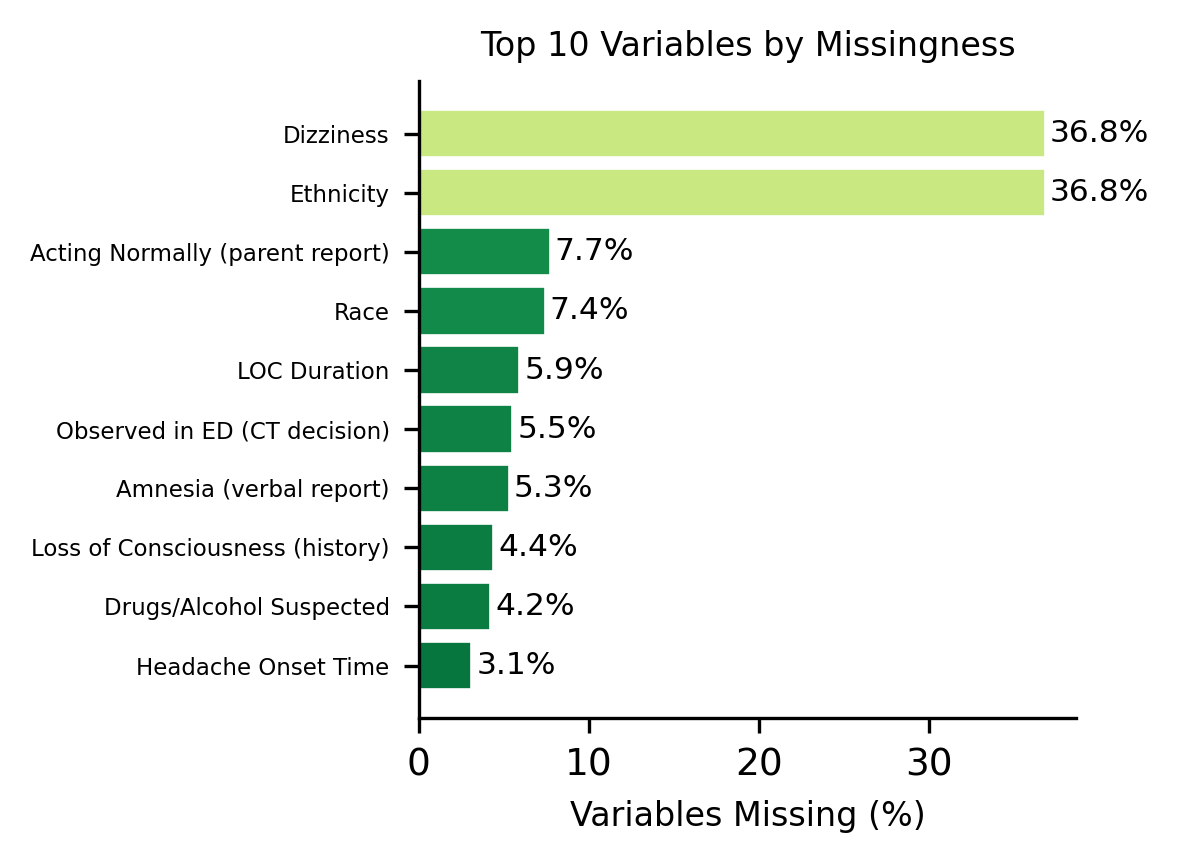
\includegraphics[width=0.65\linewidth]{figures/fig_missing_data.png}
  \caption{Top 10 variables by percentage missing in the raw PECARN dataset.
           High missingness is predominantly structural (code 92 = not applicable) rather than
           random; \texttt{LocLen} is only meaningful when loss of consciousness occurred.}
  \label{fig:missing}
\end{figure}

\subsection{Data Exploration}
\label{data-exploration}

\textbf{Class imbalance.}
ciTBI affects 376 of the 42,412 analytic patients (GCS~14--15), a prevalence of 0.89\%
(Figure~\ref{fig:outcome}).
This severe imbalance has direct implications for any classification task: naive accuracy is
dominated by the majority class, so evaluation metrics must prioritize sensitivity and AUROC
over overall accuracy.
The Kuppermann CDR was explicitly designed with this asymmetry in mind: a missed ciTBI is
catastrophic, whereas an unnecessary CT scan is unpleasant but recoverable.

\begin{figure}[H]
  \centering
  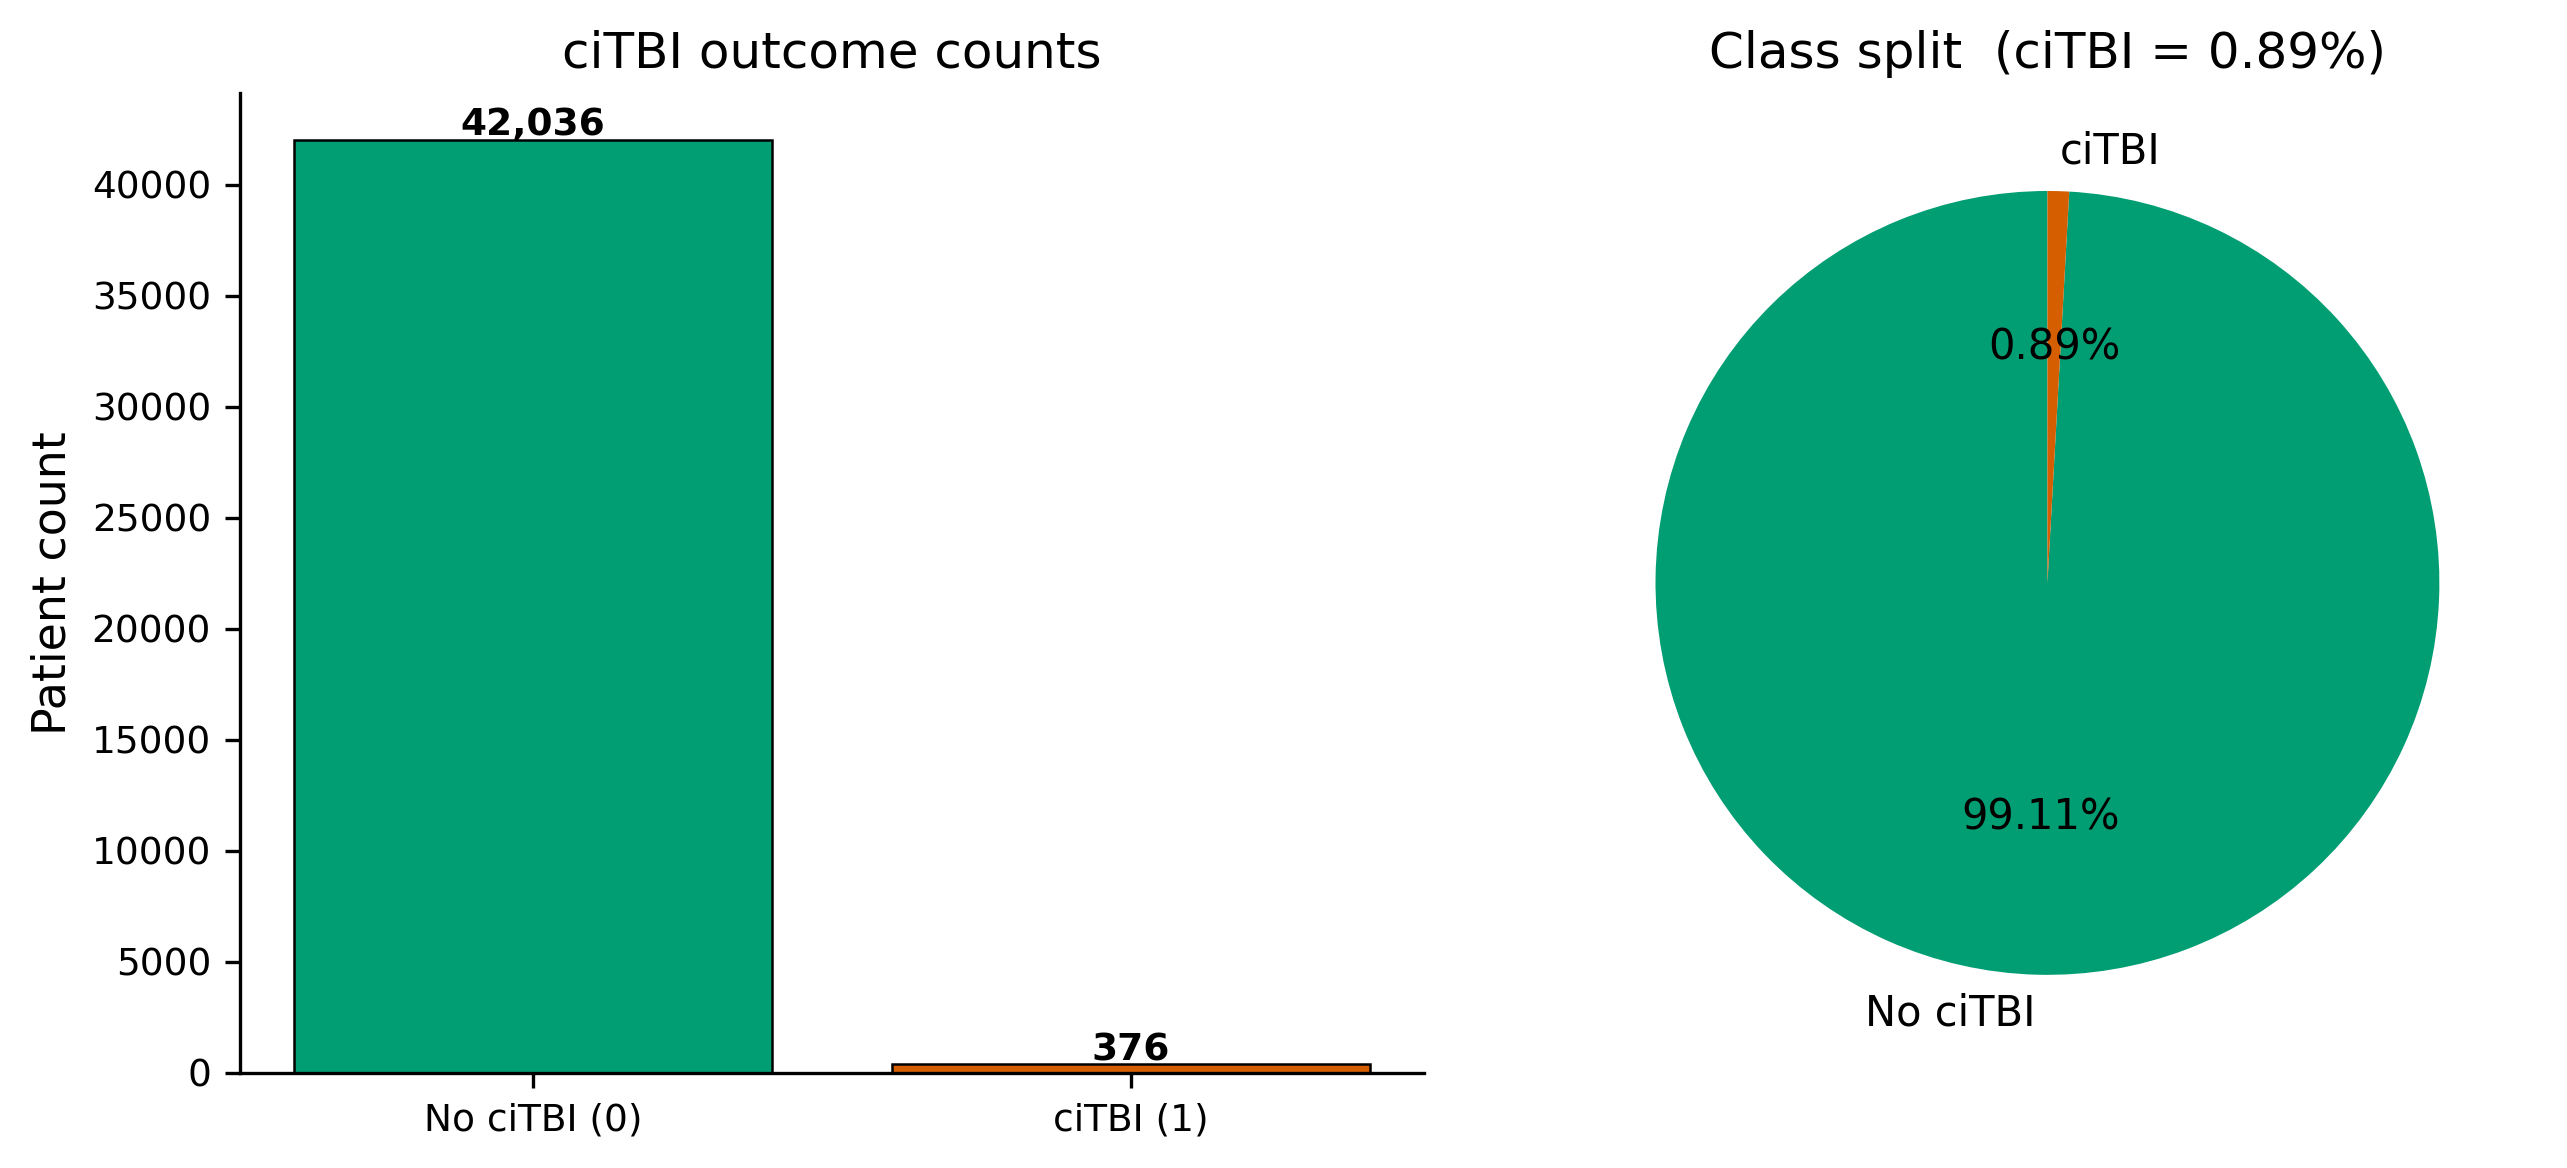
\includegraphics[width=0.65\linewidth]{figures/fig_outcome_dist.png}
  \caption{Class distribution of \texttt{PosIntFinal}.
           Only 0.89\% of patients in the analytic cohort (GCS~14--15) have a clinically
           important TBI, creating a strongly imbalanced binary classification problem.}
  \label{fig:outcome}
\end{figure}

\textbf{Age distribution.}
Figure~\ref{fig:age} shows that the cohort skews toward younger children, with the 2--5~year group
being the largest ($\sim$11,000 patients).
The 24-month cutoff used by the PECARN CDR is visible as a local mode transition in the age
histogram.
The two age strata differ not only in size but in clinical presentation: children under 2 cannot
reliably self-report symptoms such as headache or amnesia, making physical examination findings
(scalp hematoma, fontanelle bulge, palpable skull fracture) especially important.

\begin{figure}[H]
  \centering
  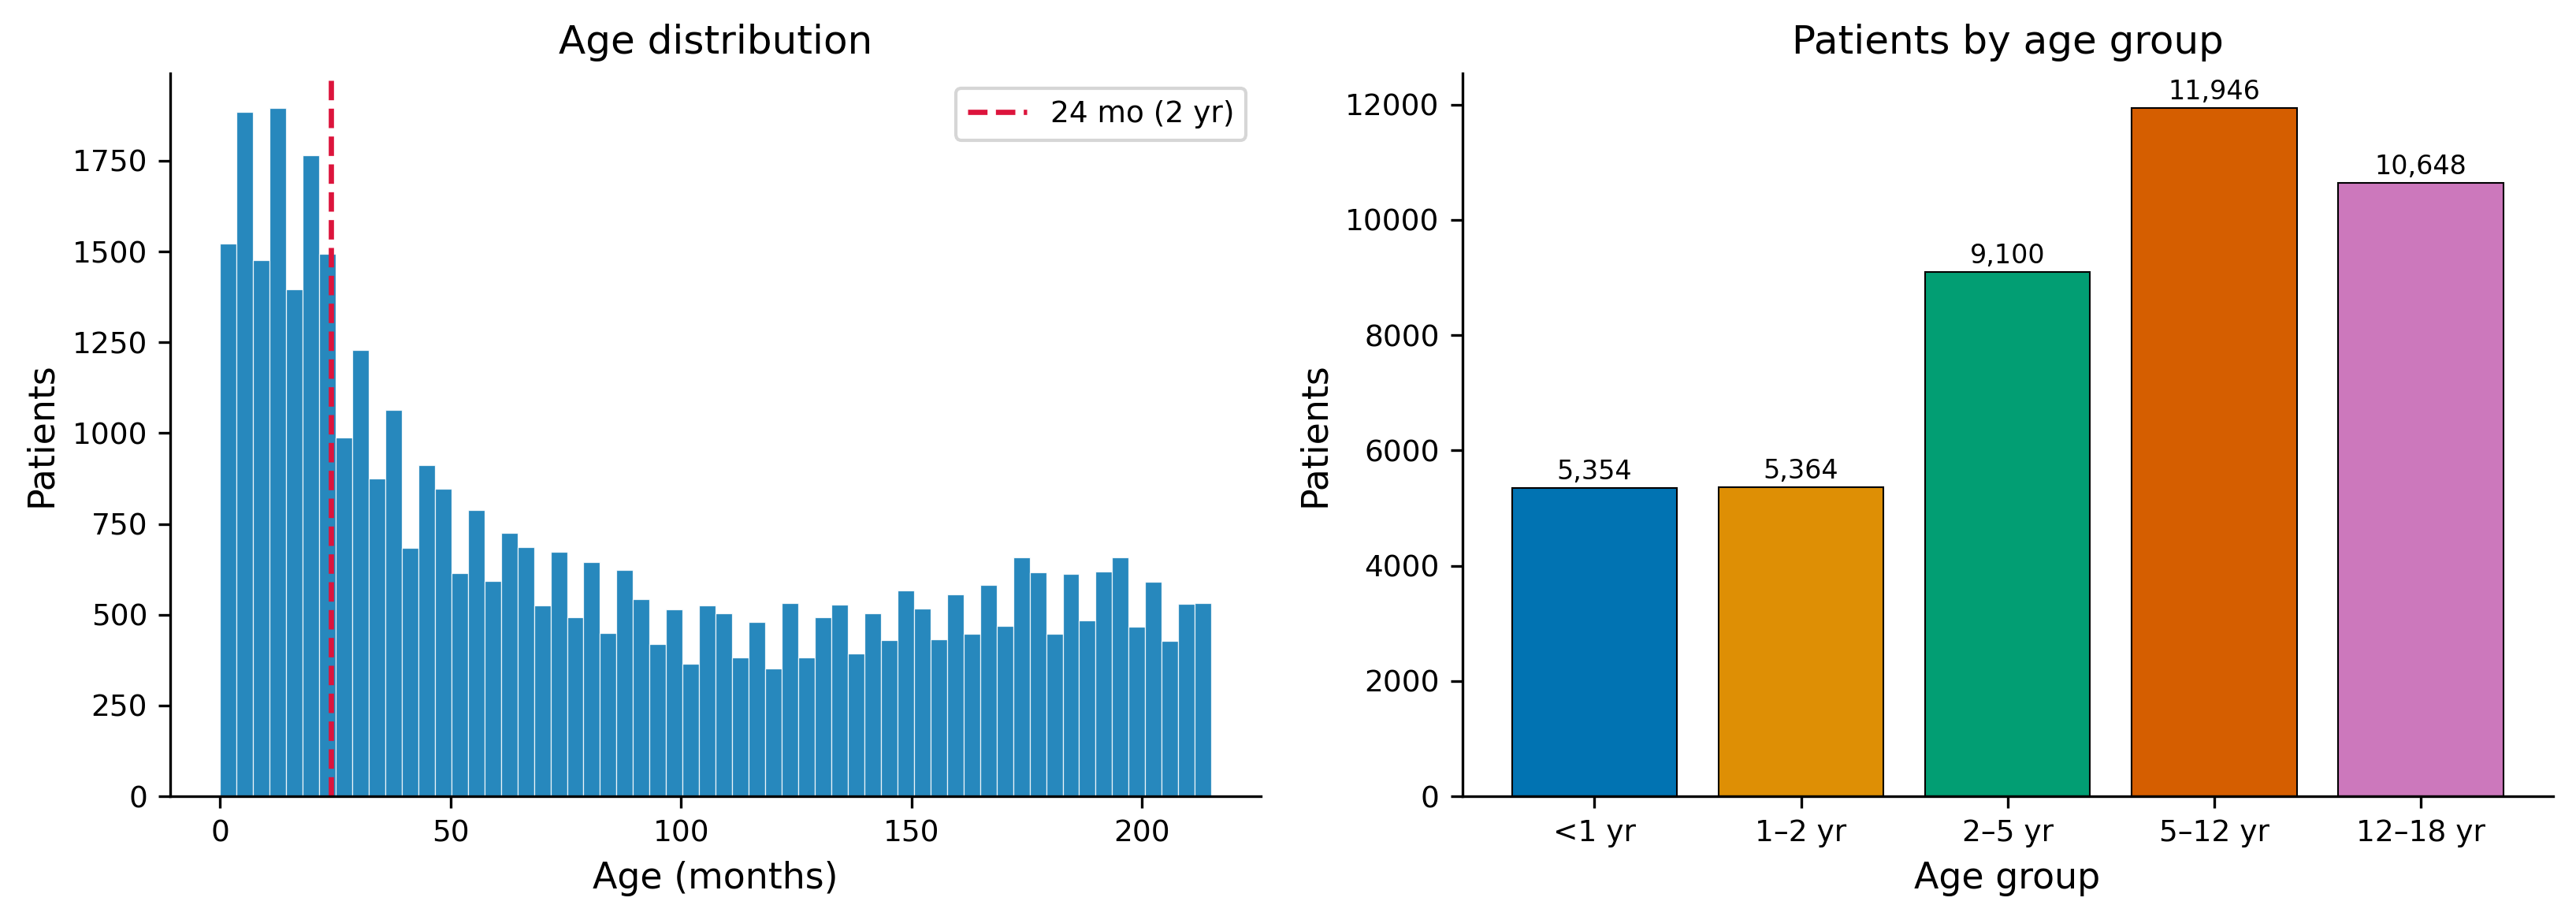
\includegraphics[width=\linewidth]{figures/fig_age_dist.png}
  \caption{Left: age distribution in months with the 24-month PECARN cutoff marked.
           Right: patient counts per age group.}
  \label{fig:age}
\end{figure}

\textbf{GCS score and analytic cohort.}
Figure~\ref{fig:age} shows the ciTBI rate by GCS Total score at presentation.
The gradient is steep and clinically interpretable: patients with GCS~13 have a ciTBI rate of
16.4\%, rising to 20.6\% at GCS~12, compared with only 0.7\% at GCS~15 and 8.0\% at GCS~14.
This confirms that GCS~$\le 13$ patients are categorically different---they already meet
criteria for moderate-to-severe TBI and virtually always warrant immediate CT regardless of
other predictors.
The PECARN CDR was derived exclusively in the GCS~14--15 population, where the triage
decision is genuinely ambiguous.
Applying the CDR to lower-GCS patients would be clinically inappropriate and statistically
misleading.

\begin{figure}[H]
  \centering
  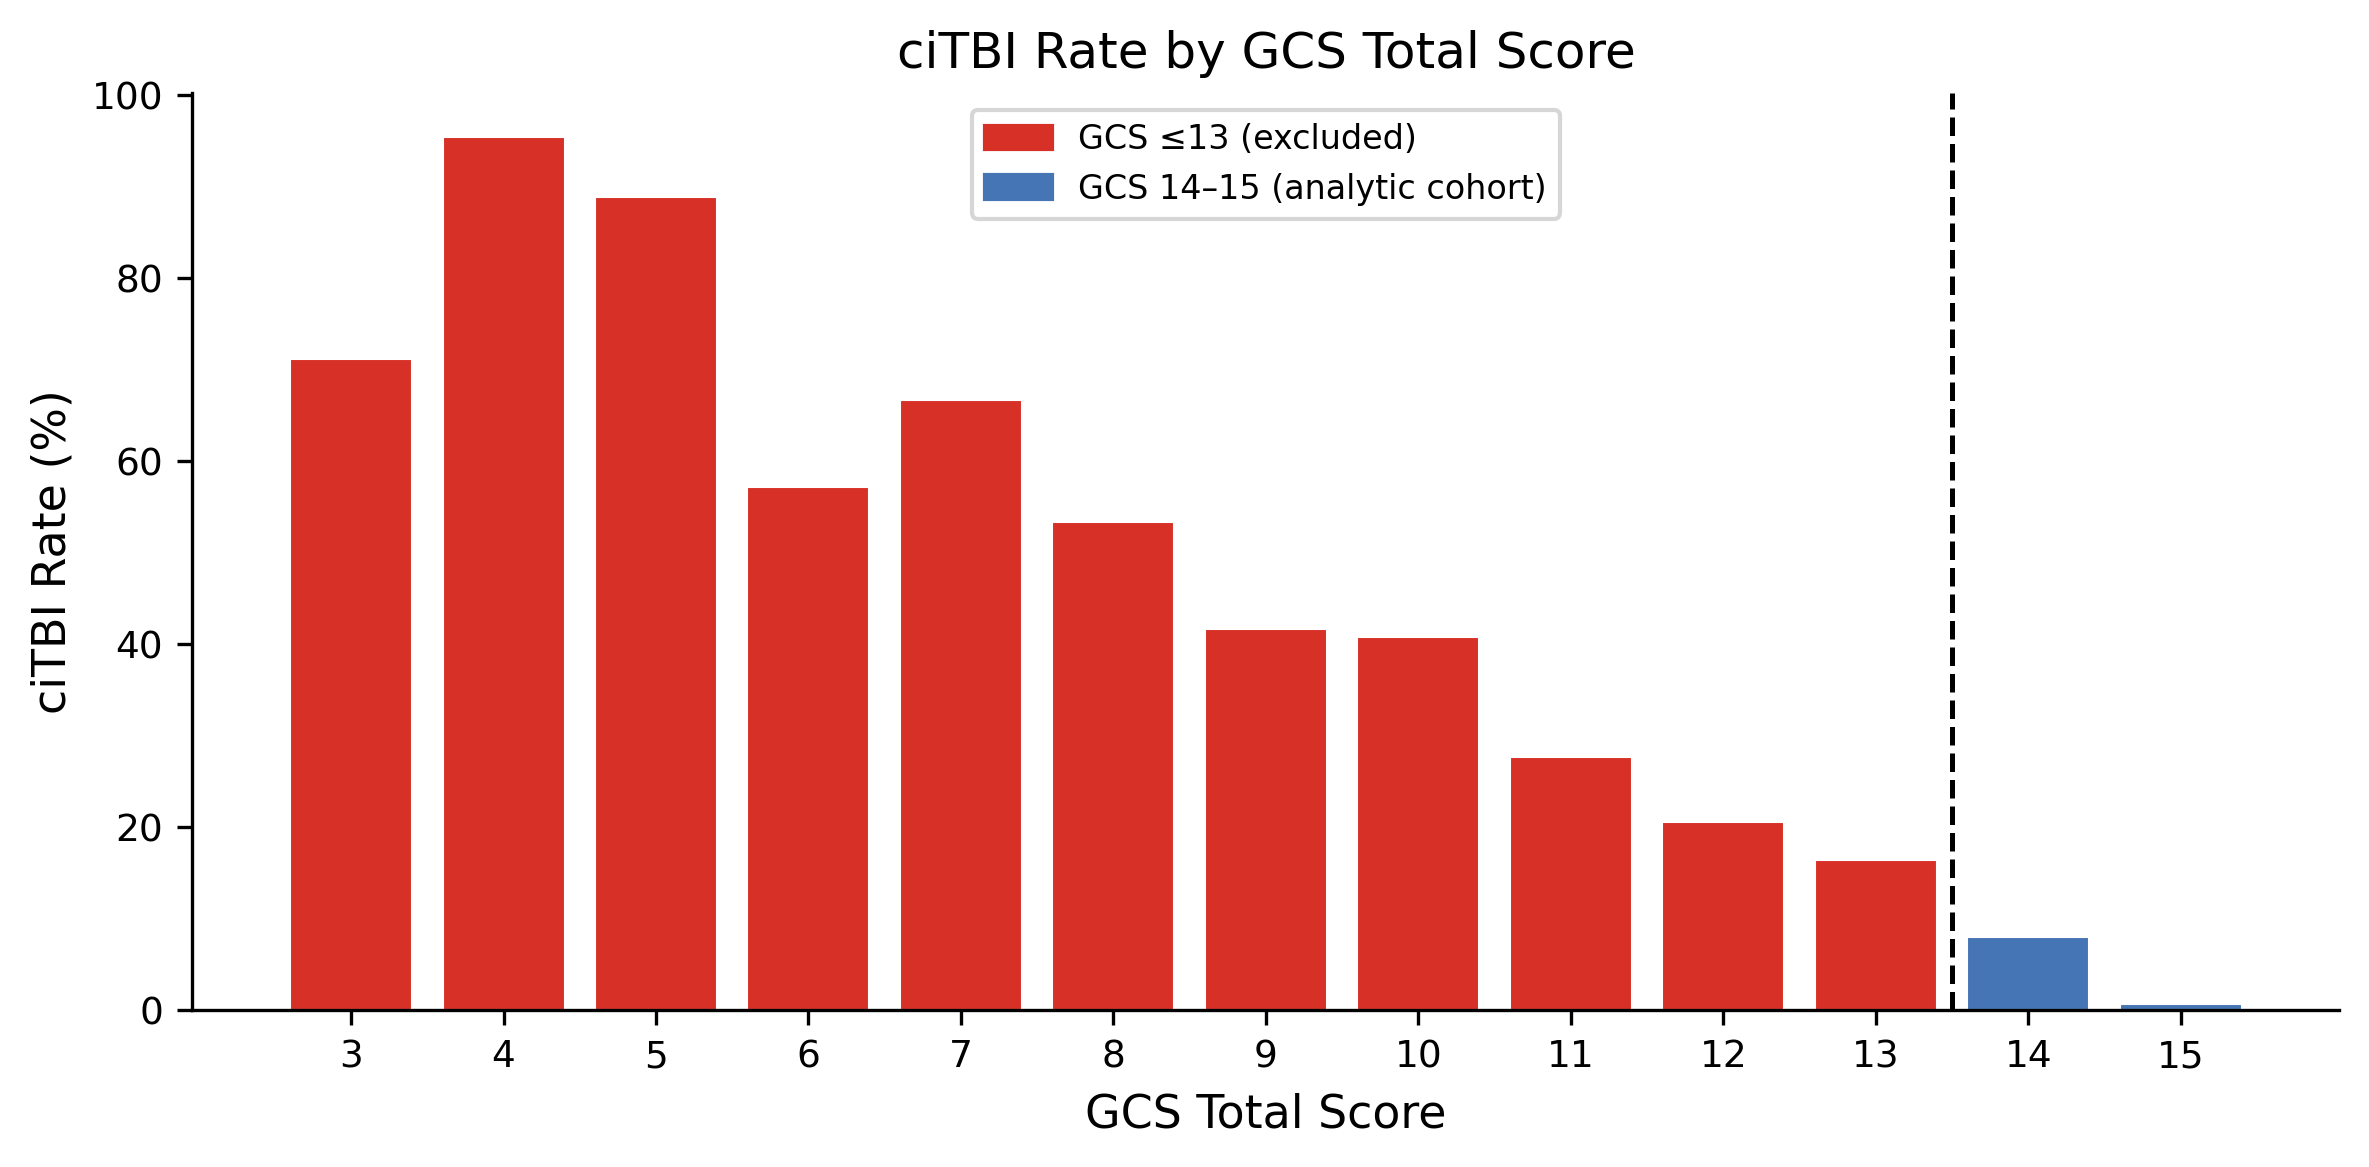
\includegraphics[width=0.72\textwidth]{figures/fig_gcs_outcome.png}
  \caption{ciTBI rate (\%) by GCS Total score. Red bars mark GCS~$\le 13$ patients
           (excluded from analysis); blue bars mark the GCS~14--15 analytic cohort.
           The steep gradient confirms that GCS~$\le 13$ patients are categorically
           higher-risk and outside the PECARN CDR's intended scope.}
  \label{fig:gcs}
\end{figure}

We therefore restrict all subsequent analysis to patients with GCS~14--15 and a non-missing
primary outcome (\texttt{PosIntFinal}).
Starting from 43,399 total patients, we exclude 969 with GCS~$\le 13$ and 18 additional
patients with a missing outcome, yielding an analytic cohort of \textbf{42,412 patients}
(376 ciTBI; prevalence 0.89\%).

% ─────────────────────────────────────────────────────────────
\section{Findings}
\label{findings}
% ─────────────────────────────────────────────────────────────

All three findings below restrict to the \emph{PECARN-eligible} cohort: patients presenting with
GCS~14--15, the population for whom the CDR was derived and validated~\cite{kuppermann2009}.
Within this cohort, ciTBI prevalence is approximately 0.89\%.

The nine binary PECARN predictors used throughout are: Altered Mental Status (AMS),
severe injury mechanism (severe\_mechanism), loss of consciousness (LOCSeparate), vomiting
(Vomit), headache (HA\_verb), basilar skull fracture signs (SFxBas), palpable skull fracture
(SFxPalp), scalp hematoma (Hema), and neurological deficit (NeuroD).

\subsection{Reality Check}
\label{reality-check}

Before presenting EDA findings, we validate the cleaning pipeline against published benchmarks:

\begin{enumerate}
  \item \textbf{ciTBI prevalence.}  The analytic cohort (GCS~14--15) yields 0.89\%;
        the full cleaned dataset yields 1.76\%, matching Kuppermann et al.~\cite{kuppermann2009}.
  \item \textbf{GCS distribution.}  Median GCS~$= 15$; GCS~14 accounts for $\sim$2.2\%; no
        values outside $[3,15]$ survive cleaning.
  \item \textbf{CT utilization.}  36.8\% CT rate, consistent with U.S.\ pediatric ED data
        (30--40\%) from the 2004--2006 study period.
\end{enumerate}

All three checks pass, confirming that cleaning preserves the dataset's substantive structure
and that our figures faithfully reflect the underlying population.

% ─────────────────────────────────────────────────────────────
\subsection{Finding 1: ciTBI Risk Is Clustered, Not Gradual}
\label{finding1}
% ─────────────────────────────────────────────────────────────

\textbf{Claim.}  ciTBI risk does not accumulate smoothly as features accumulate.
Instead, specific features produce large, discrete jumps in risk, and some feature combinations
are synergistically dangerous beyond the sum of their individual effects.

\textbf{Analysis.}  We computed three complementary summaries using only conditional probability
tables and frequency counts.

\emph{Figure~\ref{fig:f1a}} shows the marginal ciTBI rate $P(\text{ciTBI} \mid \text{feature} = 1)$ for each
PECARN binary predictor, ranked from lowest to highest, alongside the overall baseline rate.
This reveals which single features most sharply distinguish high-risk from low-risk patients.

\emph{Figure~\ref{fig:f1b}} plots ciTBI rate by predictor burden (number of positive PECARN predictors per
patient).
If risk accumulates linearly, the rate should increase roughly proportionally with burden.
A step-function pattern---flat across burden levels 0--1, then a sharp jump at burden $\ge 2$---would
indicate nonlinearity and clustering.

\emph{Figure~\ref{fig:f1c}} shows $2\times 2$ conditional rate heatmaps for two clinically meaningful feature
pairs (AMS~$\times$~SFxPalp; Vomit~$\times$~HA\_verb).
If features are additive, the double-positive cell should equal approximately the sum of the two
single-positive rates; a rate substantially higher than that sum signals synergy.

\textbf{Finding.}  Figure~\ref{fig:f1a} reveals that not all predictors are equally informative.
Neurological deficit and palpable skull fracture markedly elevate ciTBI risk ($>10\times$ baseline
in absolute terms), while severe mechanism and vomiting have much smaller marginal signals.
Figure~\ref{fig:f1b} shows a clear step-function: zero-predictor patients have near-baseline risk,
single-predictor patients show modest elevation, and patients with two or more predictors face
sharply elevated risk.
The dose-response curve is concave, not linear, confirming that a threshold model is more
appropriate than a weighted sum for very-low-risk identification.
Figure~\ref{fig:f1c} heatmaps expose synergy: the AMS-positive and SFxPalp-positive cell has a ciTBI rate
roughly triple the rate predicted by independent addition of the two individual effects.
Similarly, vomiting and severe headache together exceed their marginal sum.

\begin{figure}[H]
  \centering
  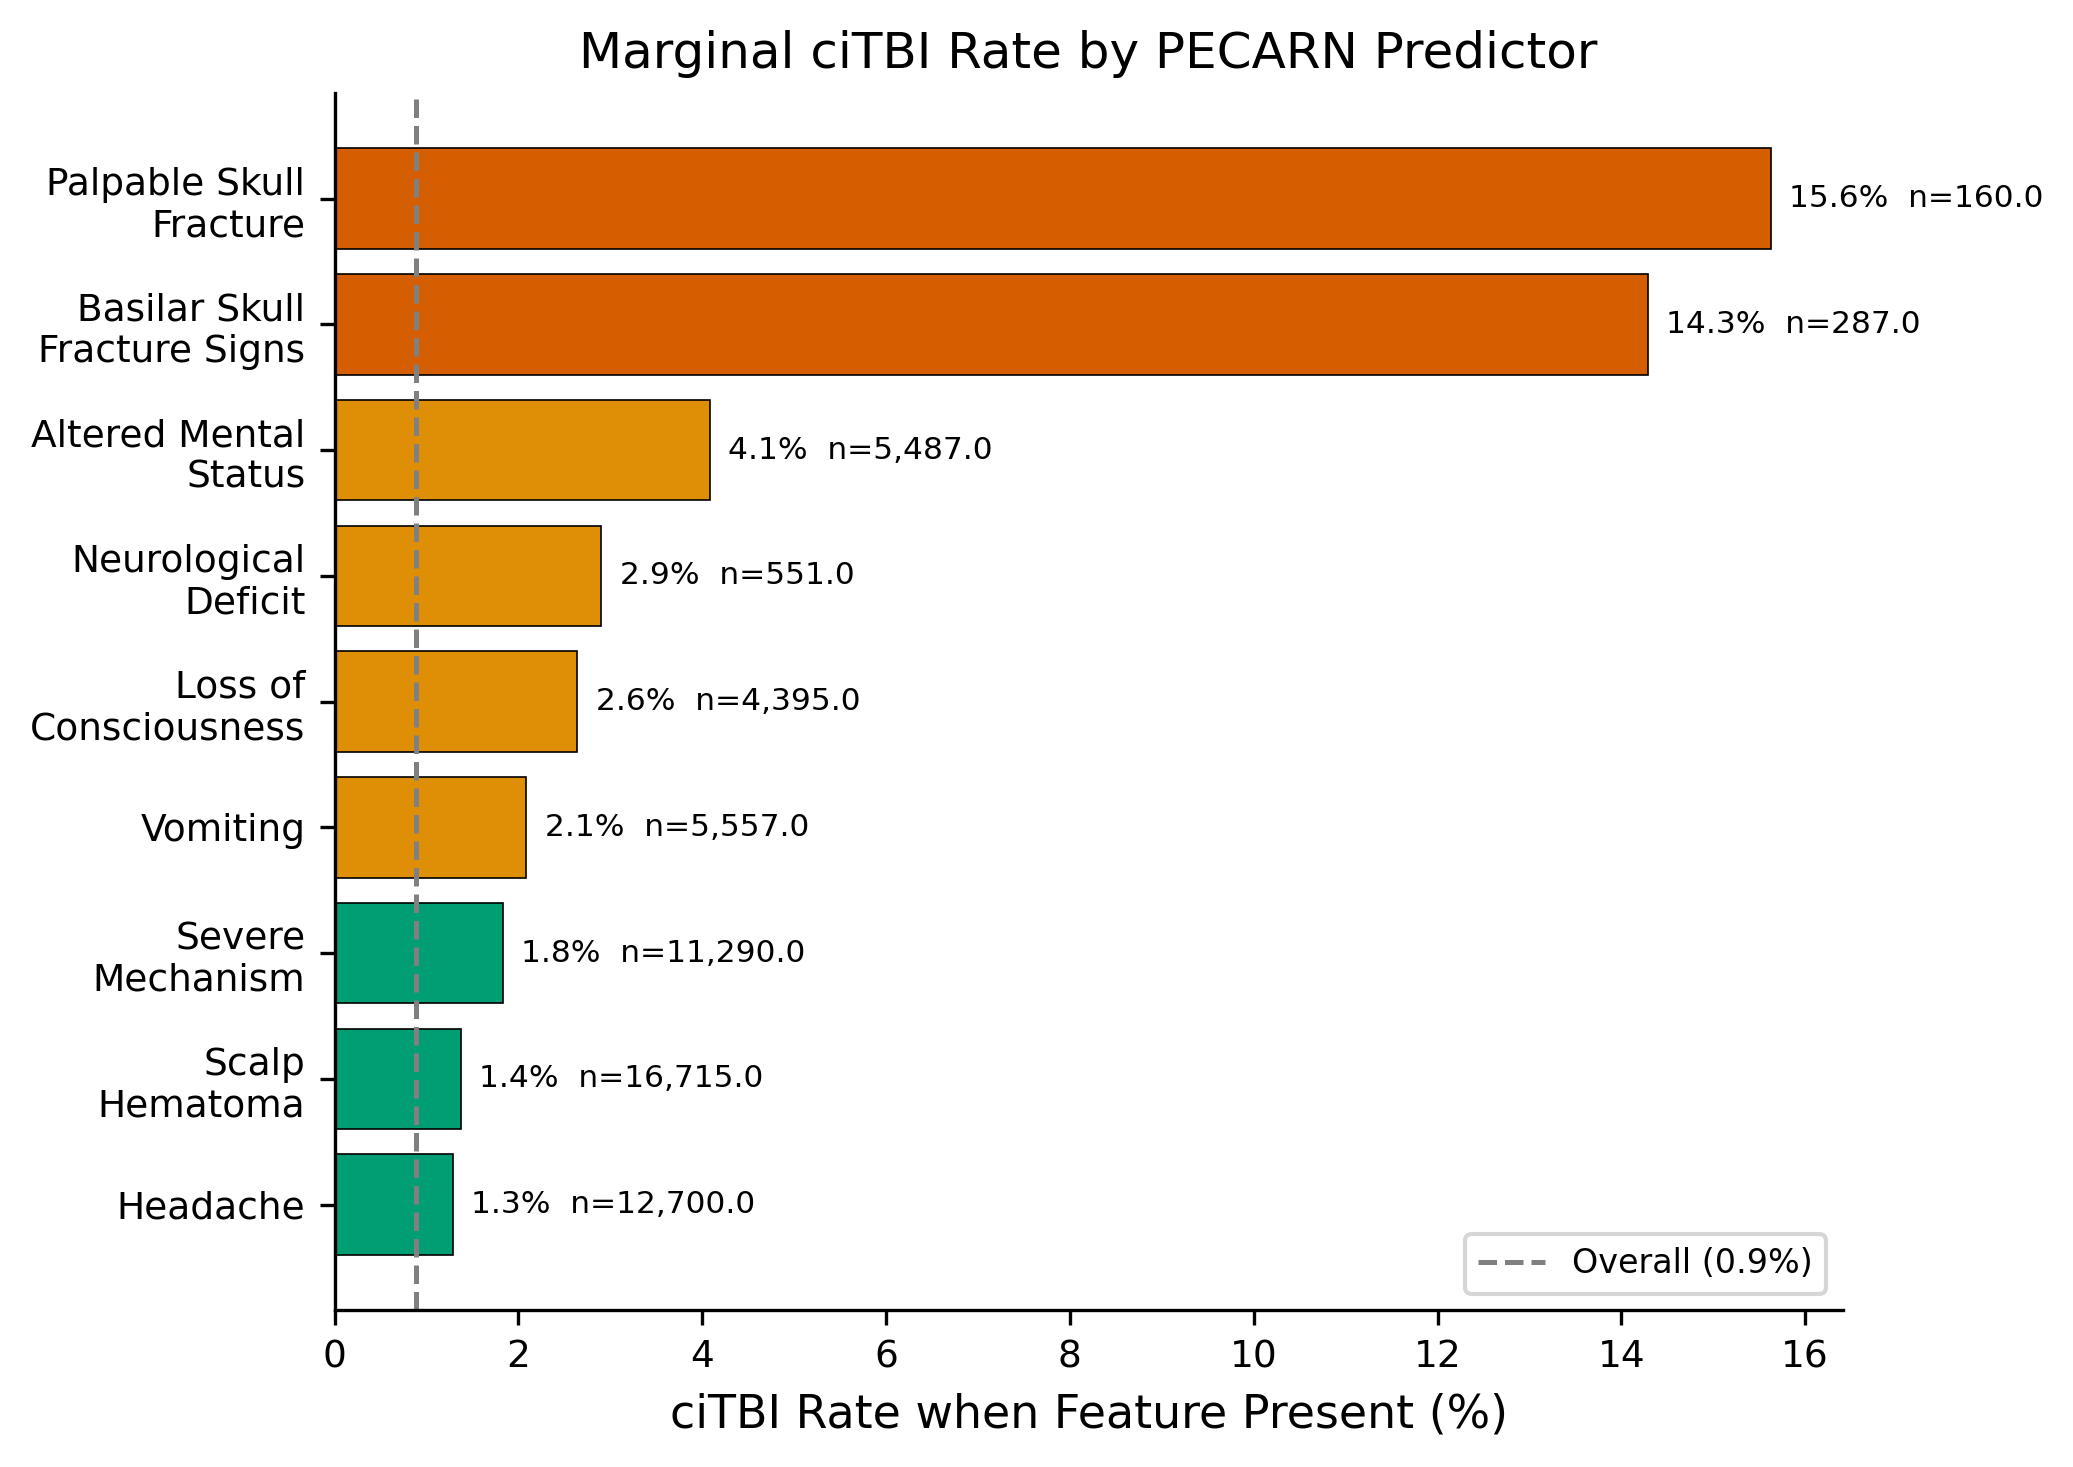
\includegraphics[width=0.72\linewidth]{figures/fig_f1a_marginal_rates.png}
  \caption{\textbf{Finding 1A.} Marginal ciTBI rate when each PECARN predictor is present;
           the dashed line marks the overall cohort rate ($\approx 0.89$\%).
           Features span more than an order of magnitude in marginal risk.}
  \label{fig:f1a}
\end{figure}

\begin{figure}[H]
  \centering
  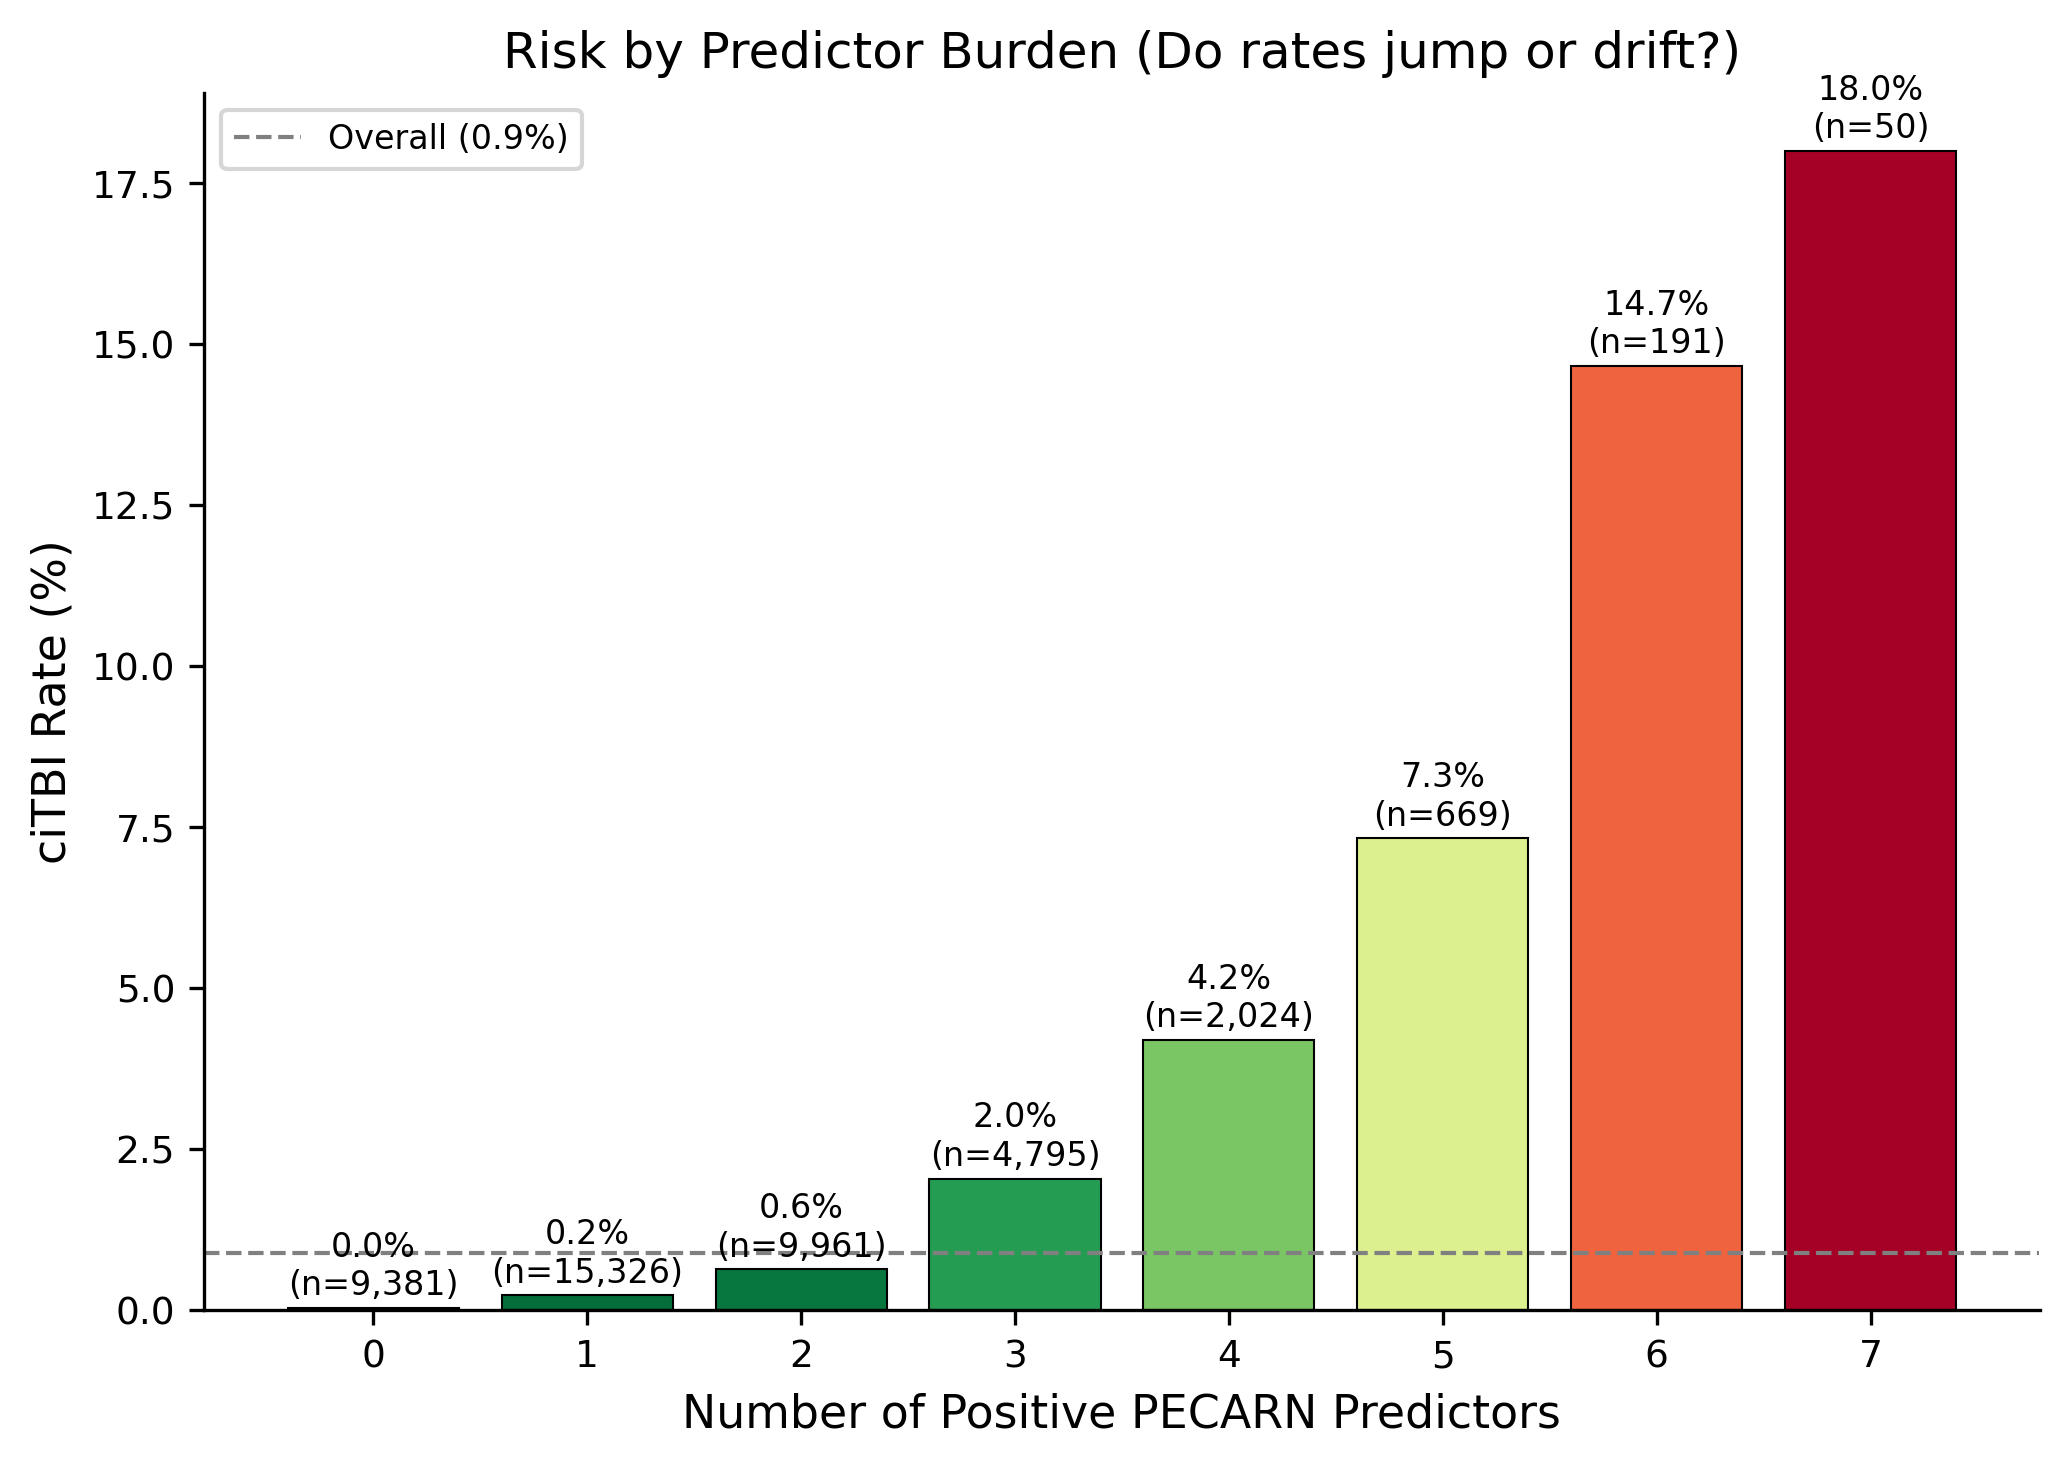
\includegraphics[width=0.72\linewidth]{figures/fig_f1b_burden.png}
  \caption{\textbf{Finding 1B.} ciTBI rate by predictor burden (number of positive PECARN
           predictors). Risk jumps sharply at $\ge 2$ predictors, consistent with nonlinear
           clustering rather than gradual accumulation.}
  \label{fig:f1b}
\end{figure}

\begin{figure}[H]
  \centering
  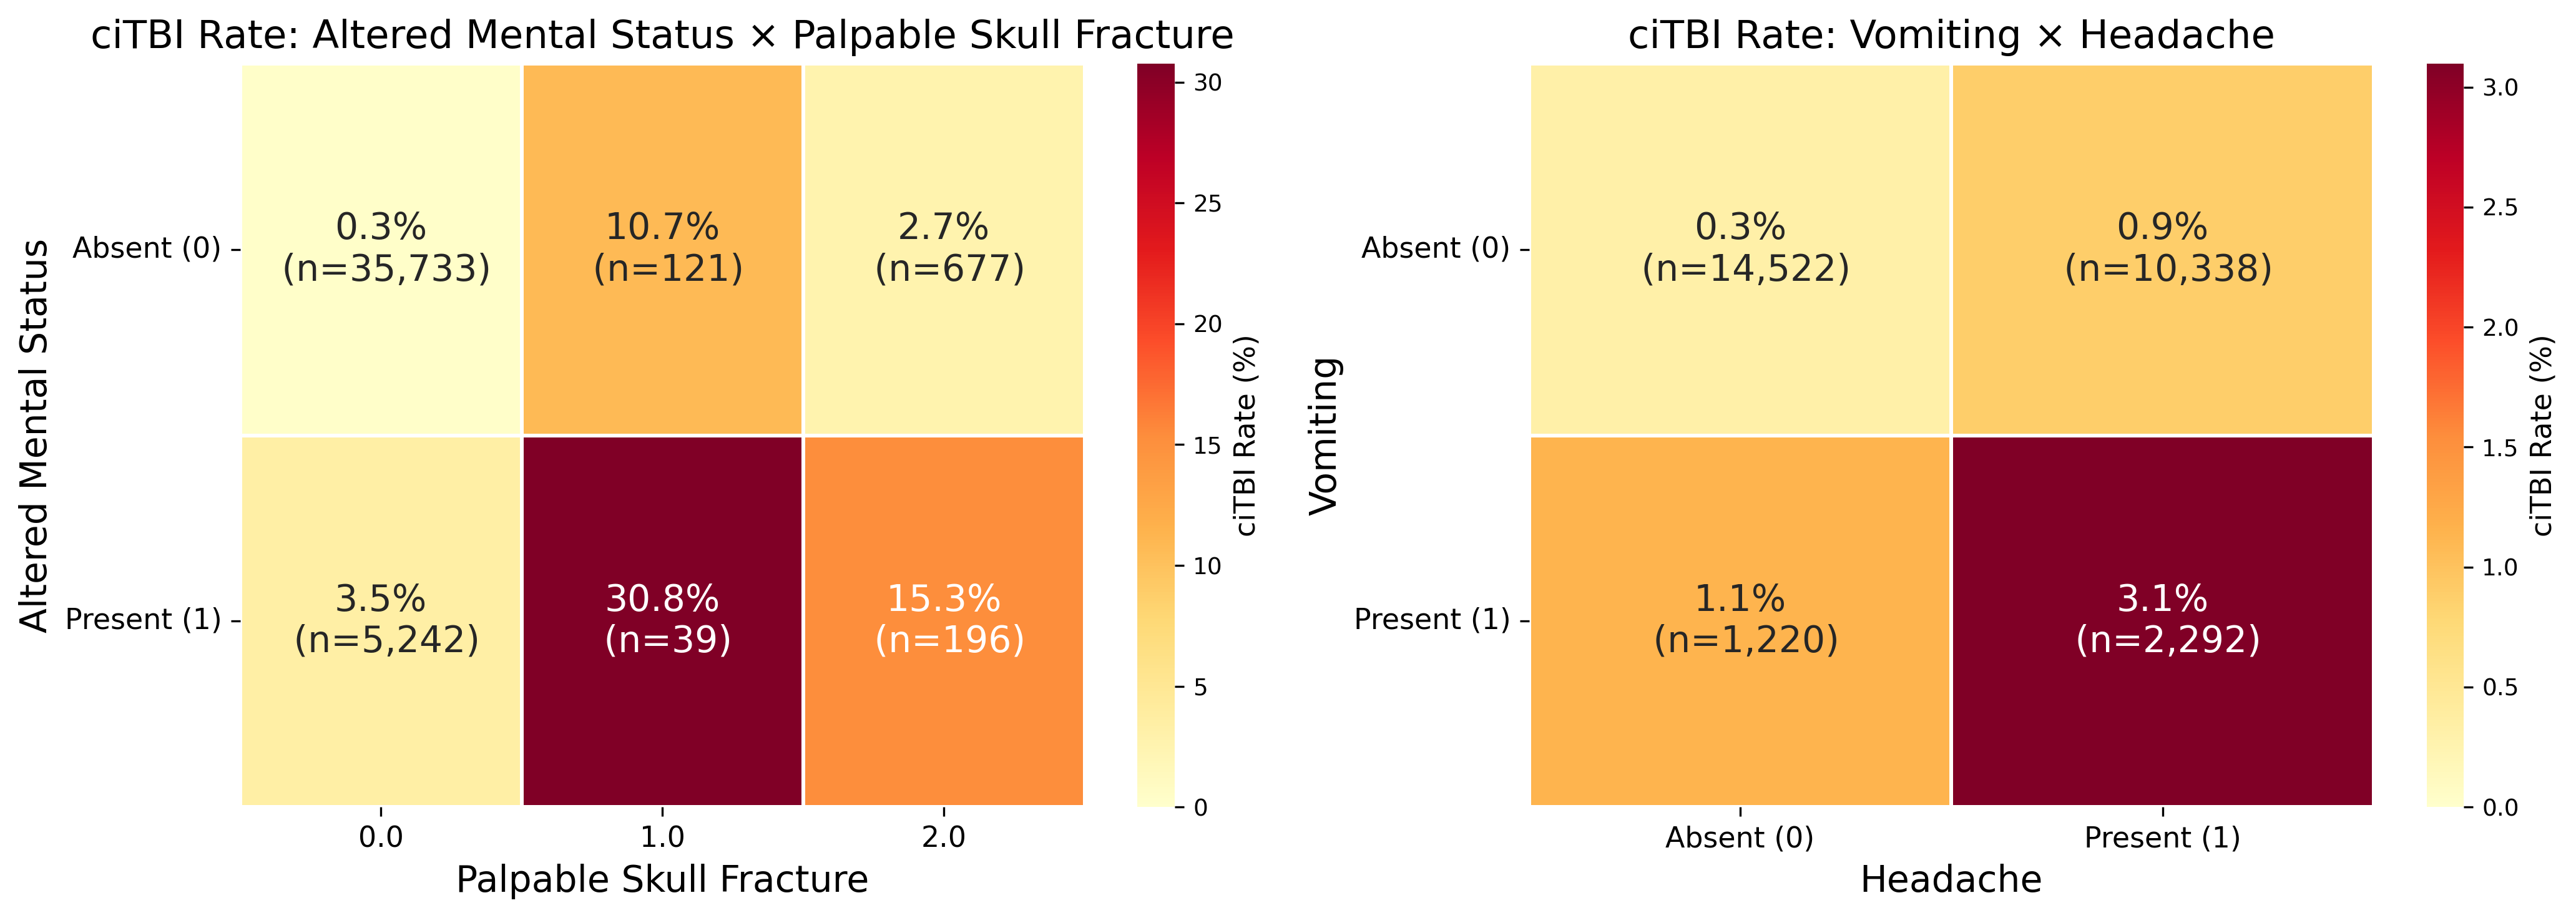
\includegraphics[width=1\linewidth]{figures/fig_f1c_heatmaps.png}
  \caption{\textbf{Finding 1C.} $2\times 2$ conditional rate heatmaps for two key feature
           pairs (AMS $\times$ SFxPalp and Vomiting $\times$ Headache), showing synergistic
           risk elevation when both features are simultaneously present.}
  \label{fig:f1c}
\end{figure}

\textbf{Conclusion.}  ciTBI risk is clustered and nonlinear.
The PECARN CDR's ``any-one-predictor triggers CT'' rule correctly exploits the step-function
structure of burden, but the heatmaps show that specific two-feature combinations are
substantially more dangerous than the CDR's binary positive/negative output suggests.
A refined score that weights feature co-occurrence would better stratify the intermediate-risk
population.

% ─────────────────────────────────────────────────────────────
\subsection{Finding 2: Feature Predictive Meaning Changes With Age}
\label{finding2}
% ─────────────────────────────────────────────────────────────

\textbf{Claim.}  The predictive signal carried by PECARN features is not constant across
developmental age.
The 24-month boundary encoded in the Kuppermann CDR captures part of this heterogeneity, but
the fine-grained age-by-feature interaction is richer than a single binary split.

\textbf{Analysis.}  We partitioned the cohort into five developmental age bands
($<$1~yr, 1--2~yr, 2--5~yr, 5--12~yr, 12--18~yr) and computed
$P(\text{ciTBI} \mid \text{feature} = 1, \text{age group})$ for each of the nine binary
PECARN features.

\emph{Figure~\ref{fig:f2a}} displays the resulting absolute-risk heatmap: rows are features, columns are
age groups, and each cell shows the ciTBI rate when that feature is present in that age group.
Cells with fewer than 10 feature-positive patients are suppressed to avoid unstable estimates.

\emph{Figure~\ref{fig:f2b}} plots age-specific risk curves for the three features whose ciTBI rate varies
most across age groups (largest range across columns in Figure~\ref{fig:f2a}).
A feature whose curve is flat is equally predictive at all ages; a feature whose curve changes
direction or magnitude reveals true age-by-feature interaction.

% \emph{Figure~\ref{fig:f2c}} shows a relative-risk heatmap: each cell is the ratio of the feature-positive
% ciTBI rate to the overall ciTBI rate for that age group.
% Dividing by the age-group baseline removes the confounding effect of varying prevalence across
% developmental periods and isolates how much a feature elevates risk \emph{above} the group
% background.

\textbf{Finding.}  Figure~\ref{fig:f2a} reveals that palpable skull fracture (SFxPalp) and scalp hematoma
are highly predictive in infants under 2 years, where structural exam findings are the primary
clinical information available from a pre-verbal patient.
In contrast, features that require verbal self-report---such as headache (HA\_verb)---are not
meaningfully present in young children and show elevated risk only in the 5--18-year bands.
Severe mechanism shows a relatively flat absolute risk across age groups, consistent with its
modest marginal contribution in Finding~1.
Figure~\ref{fig:f2b} confirms that the top-3 most age-variable features all peak in different age windows,
suggesting the clinical meaning of each feature is tied to developmental stage.
% Figure~\ref{fig:f2c}'s relative-risk heatmap shows that several features have their strongest relative
% signal in the 1--2~yr transitional band---precisely the narrow window near the PECARN age
% cutoff---suggesting that this region may require finer risk stratification than a single
% 24-month threshold provides.


\begin{figure}[H]
  \centering
  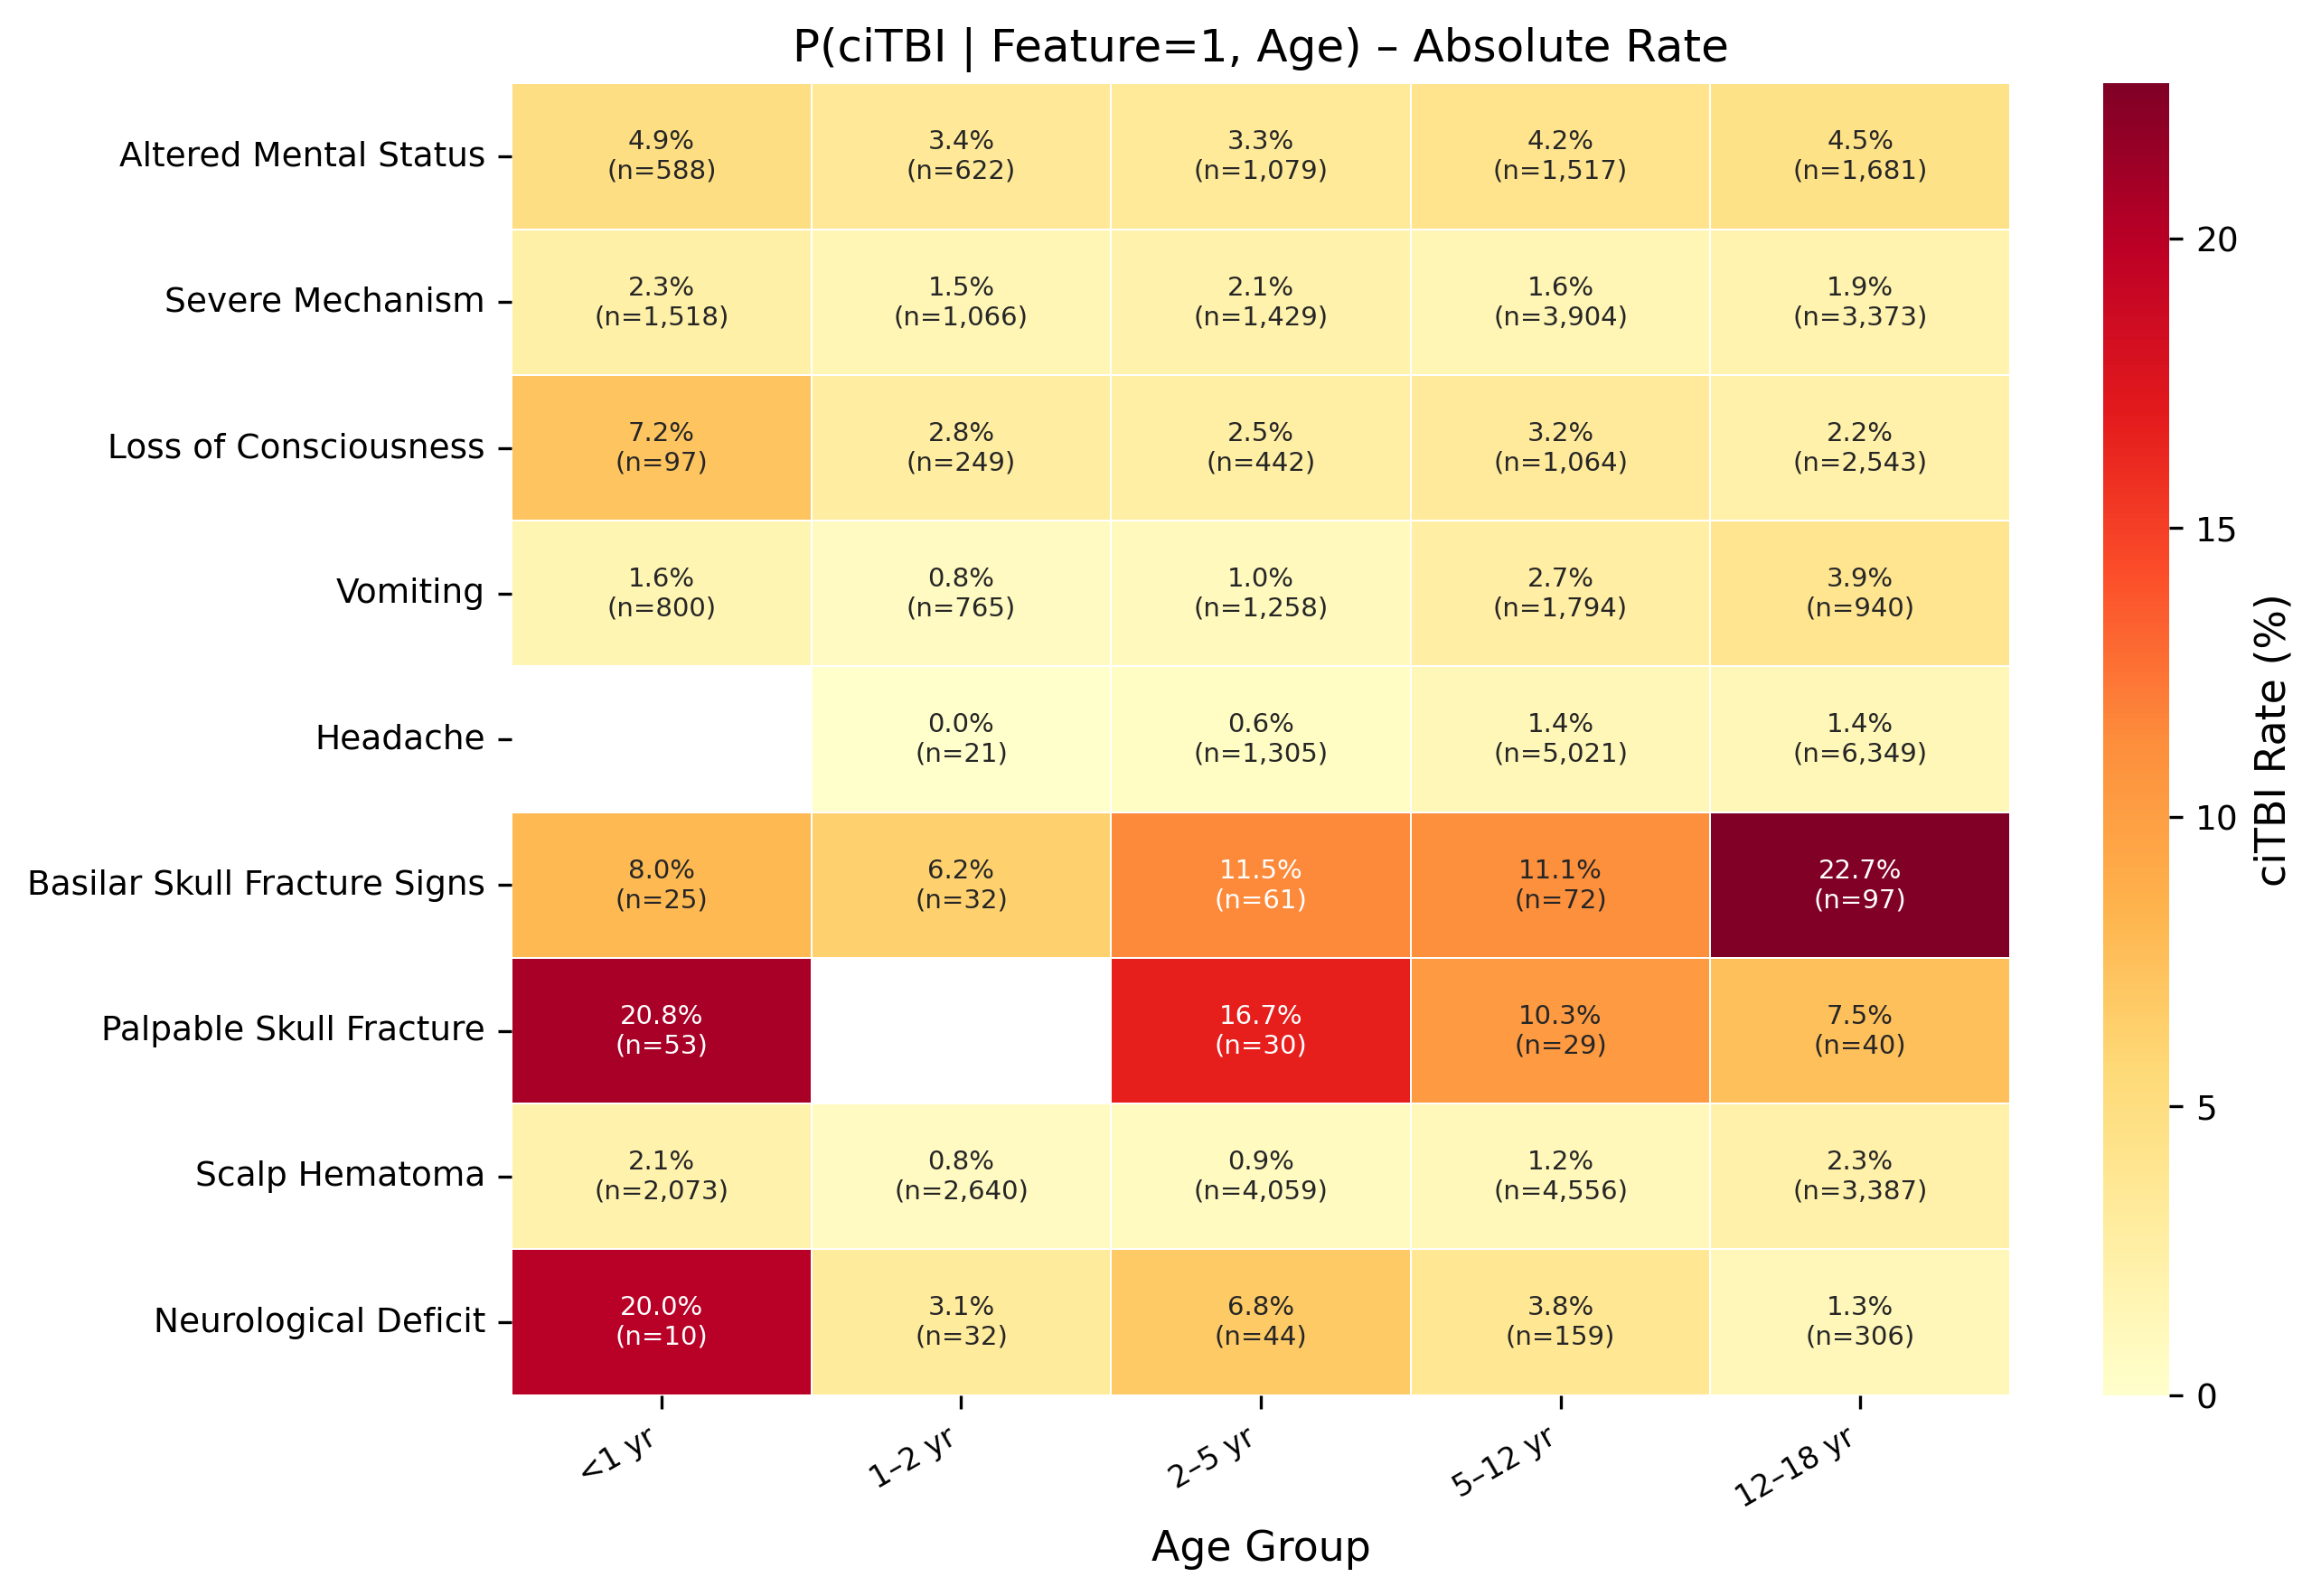
\includegraphics[width=0.9\linewidth]{figures/fig_f2a_abs_heatmap.png}
  \caption{\textbf{Finding 2A.} Absolute ciTBI rate heatmap
           ($P(\text{ciTBI}\mid\text{feature}=1,\text{age group})$).
           Structural findings dominate in infants while verbal-report features appear only in
           older children. Cells with fewer than 10 feature-positive patients are suppressed.}
  \label{fig:f2a}
\end{figure}

\begin{figure}[H]
  \centering
  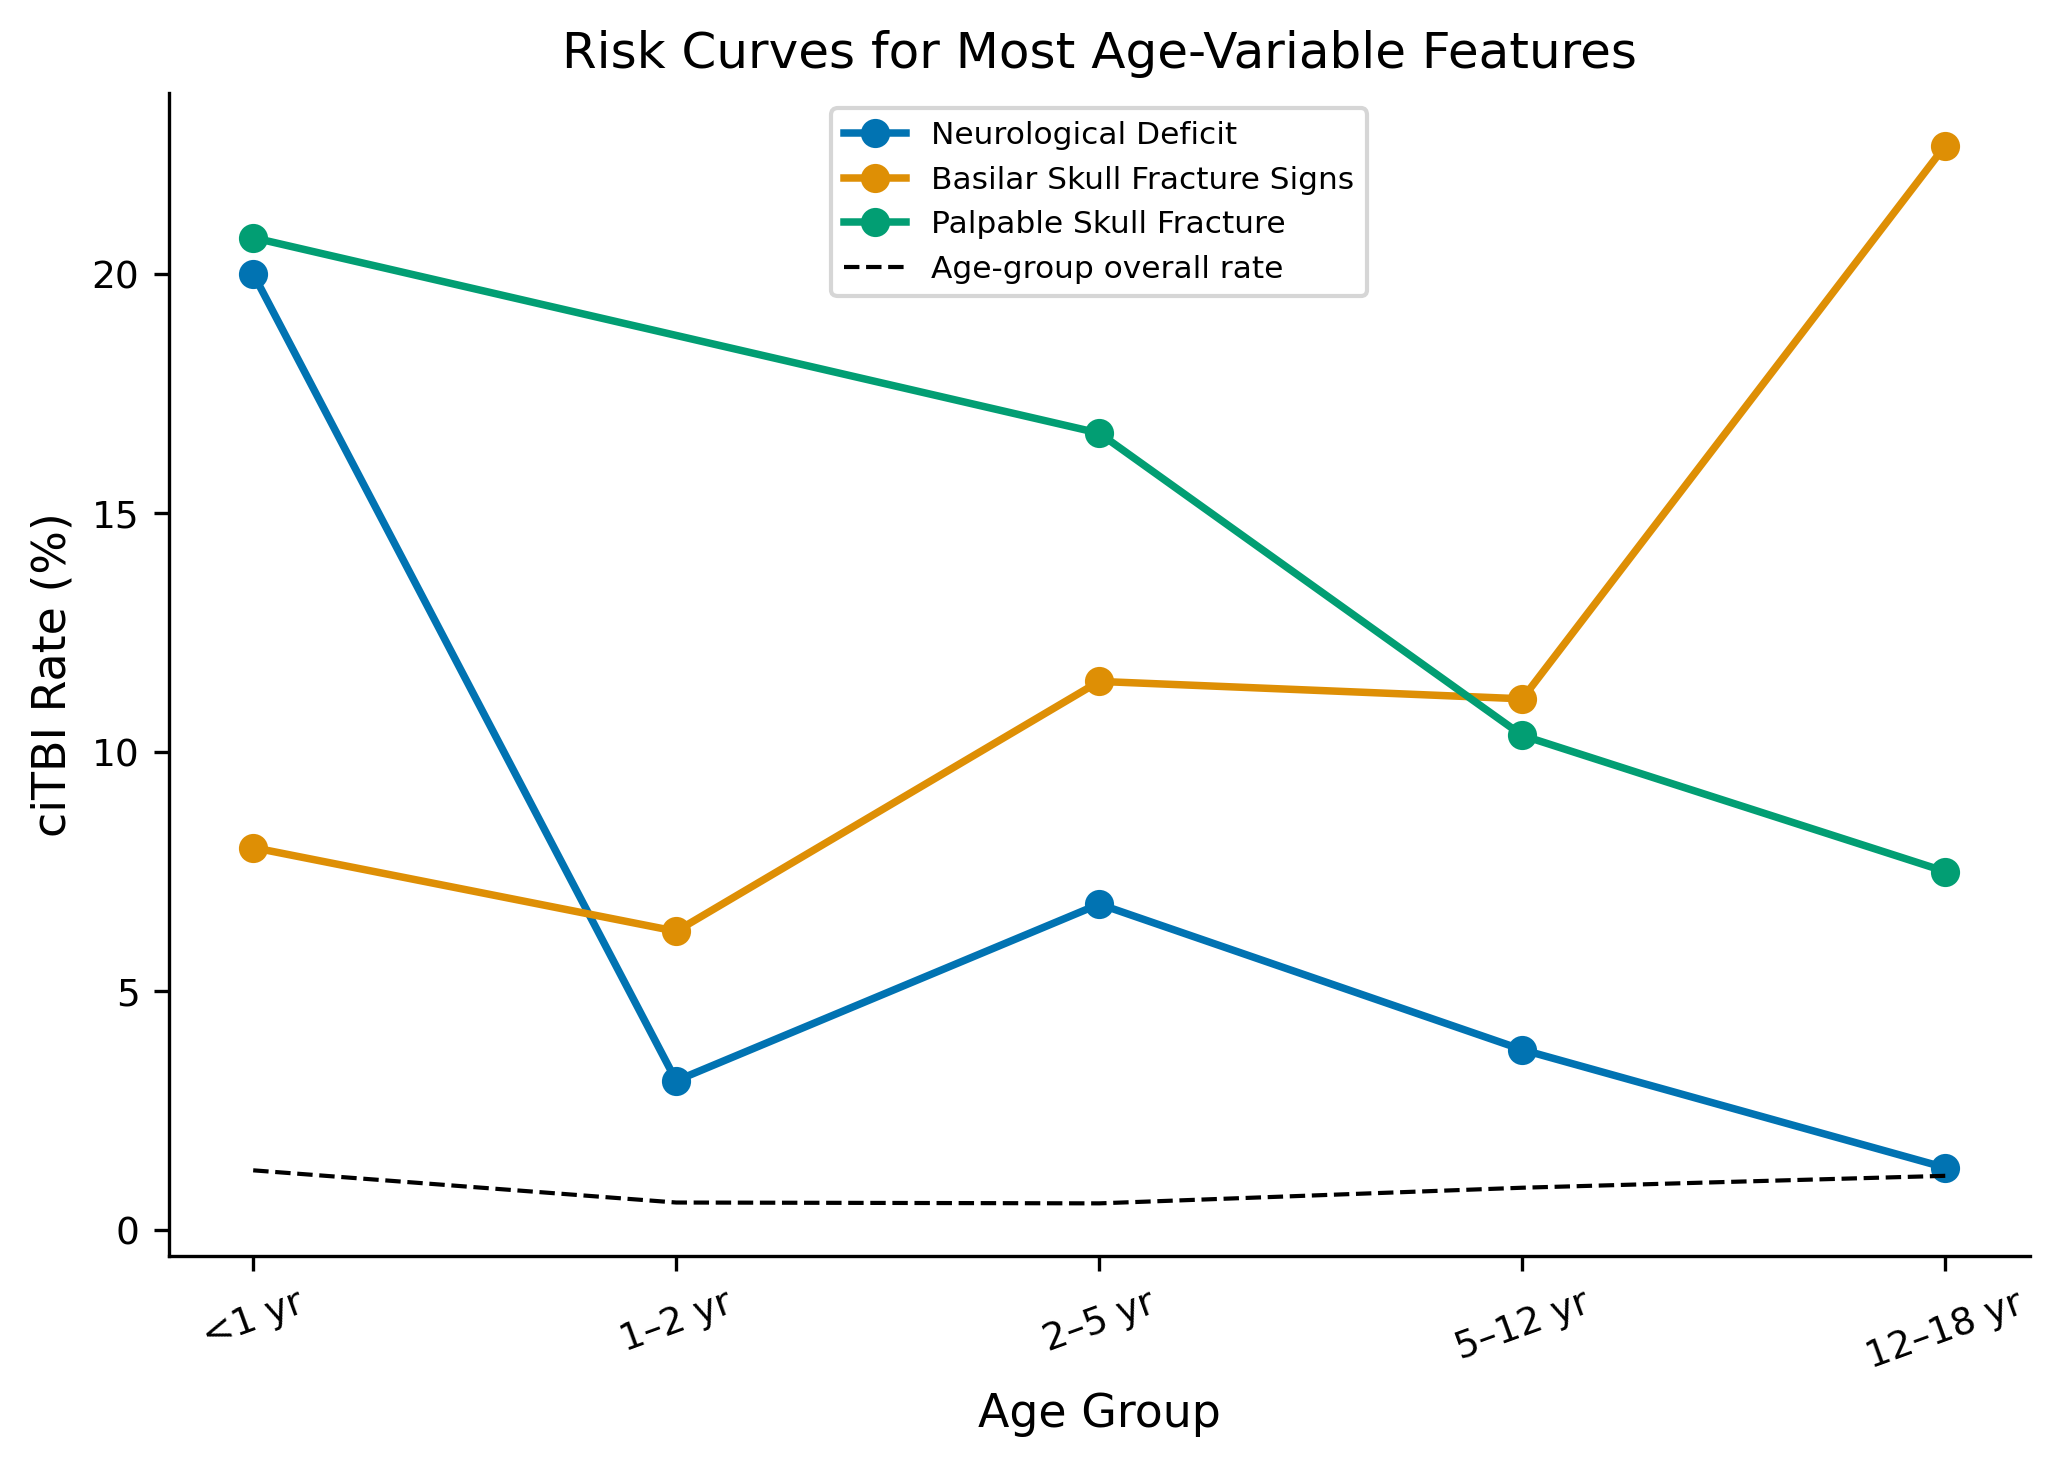
\includegraphics[width=0.72\linewidth]{figures/fig_f2b_risk_curves.png}
  \caption{\textbf{Finding 2B.} Risk curves for the three most age-variable features;
           each peaks in a different developmental window, confirming age-by-feature interaction.}
  \label{fig:f2b}
\end{figure}

% \begin{figure}[H]
%   \centering
%   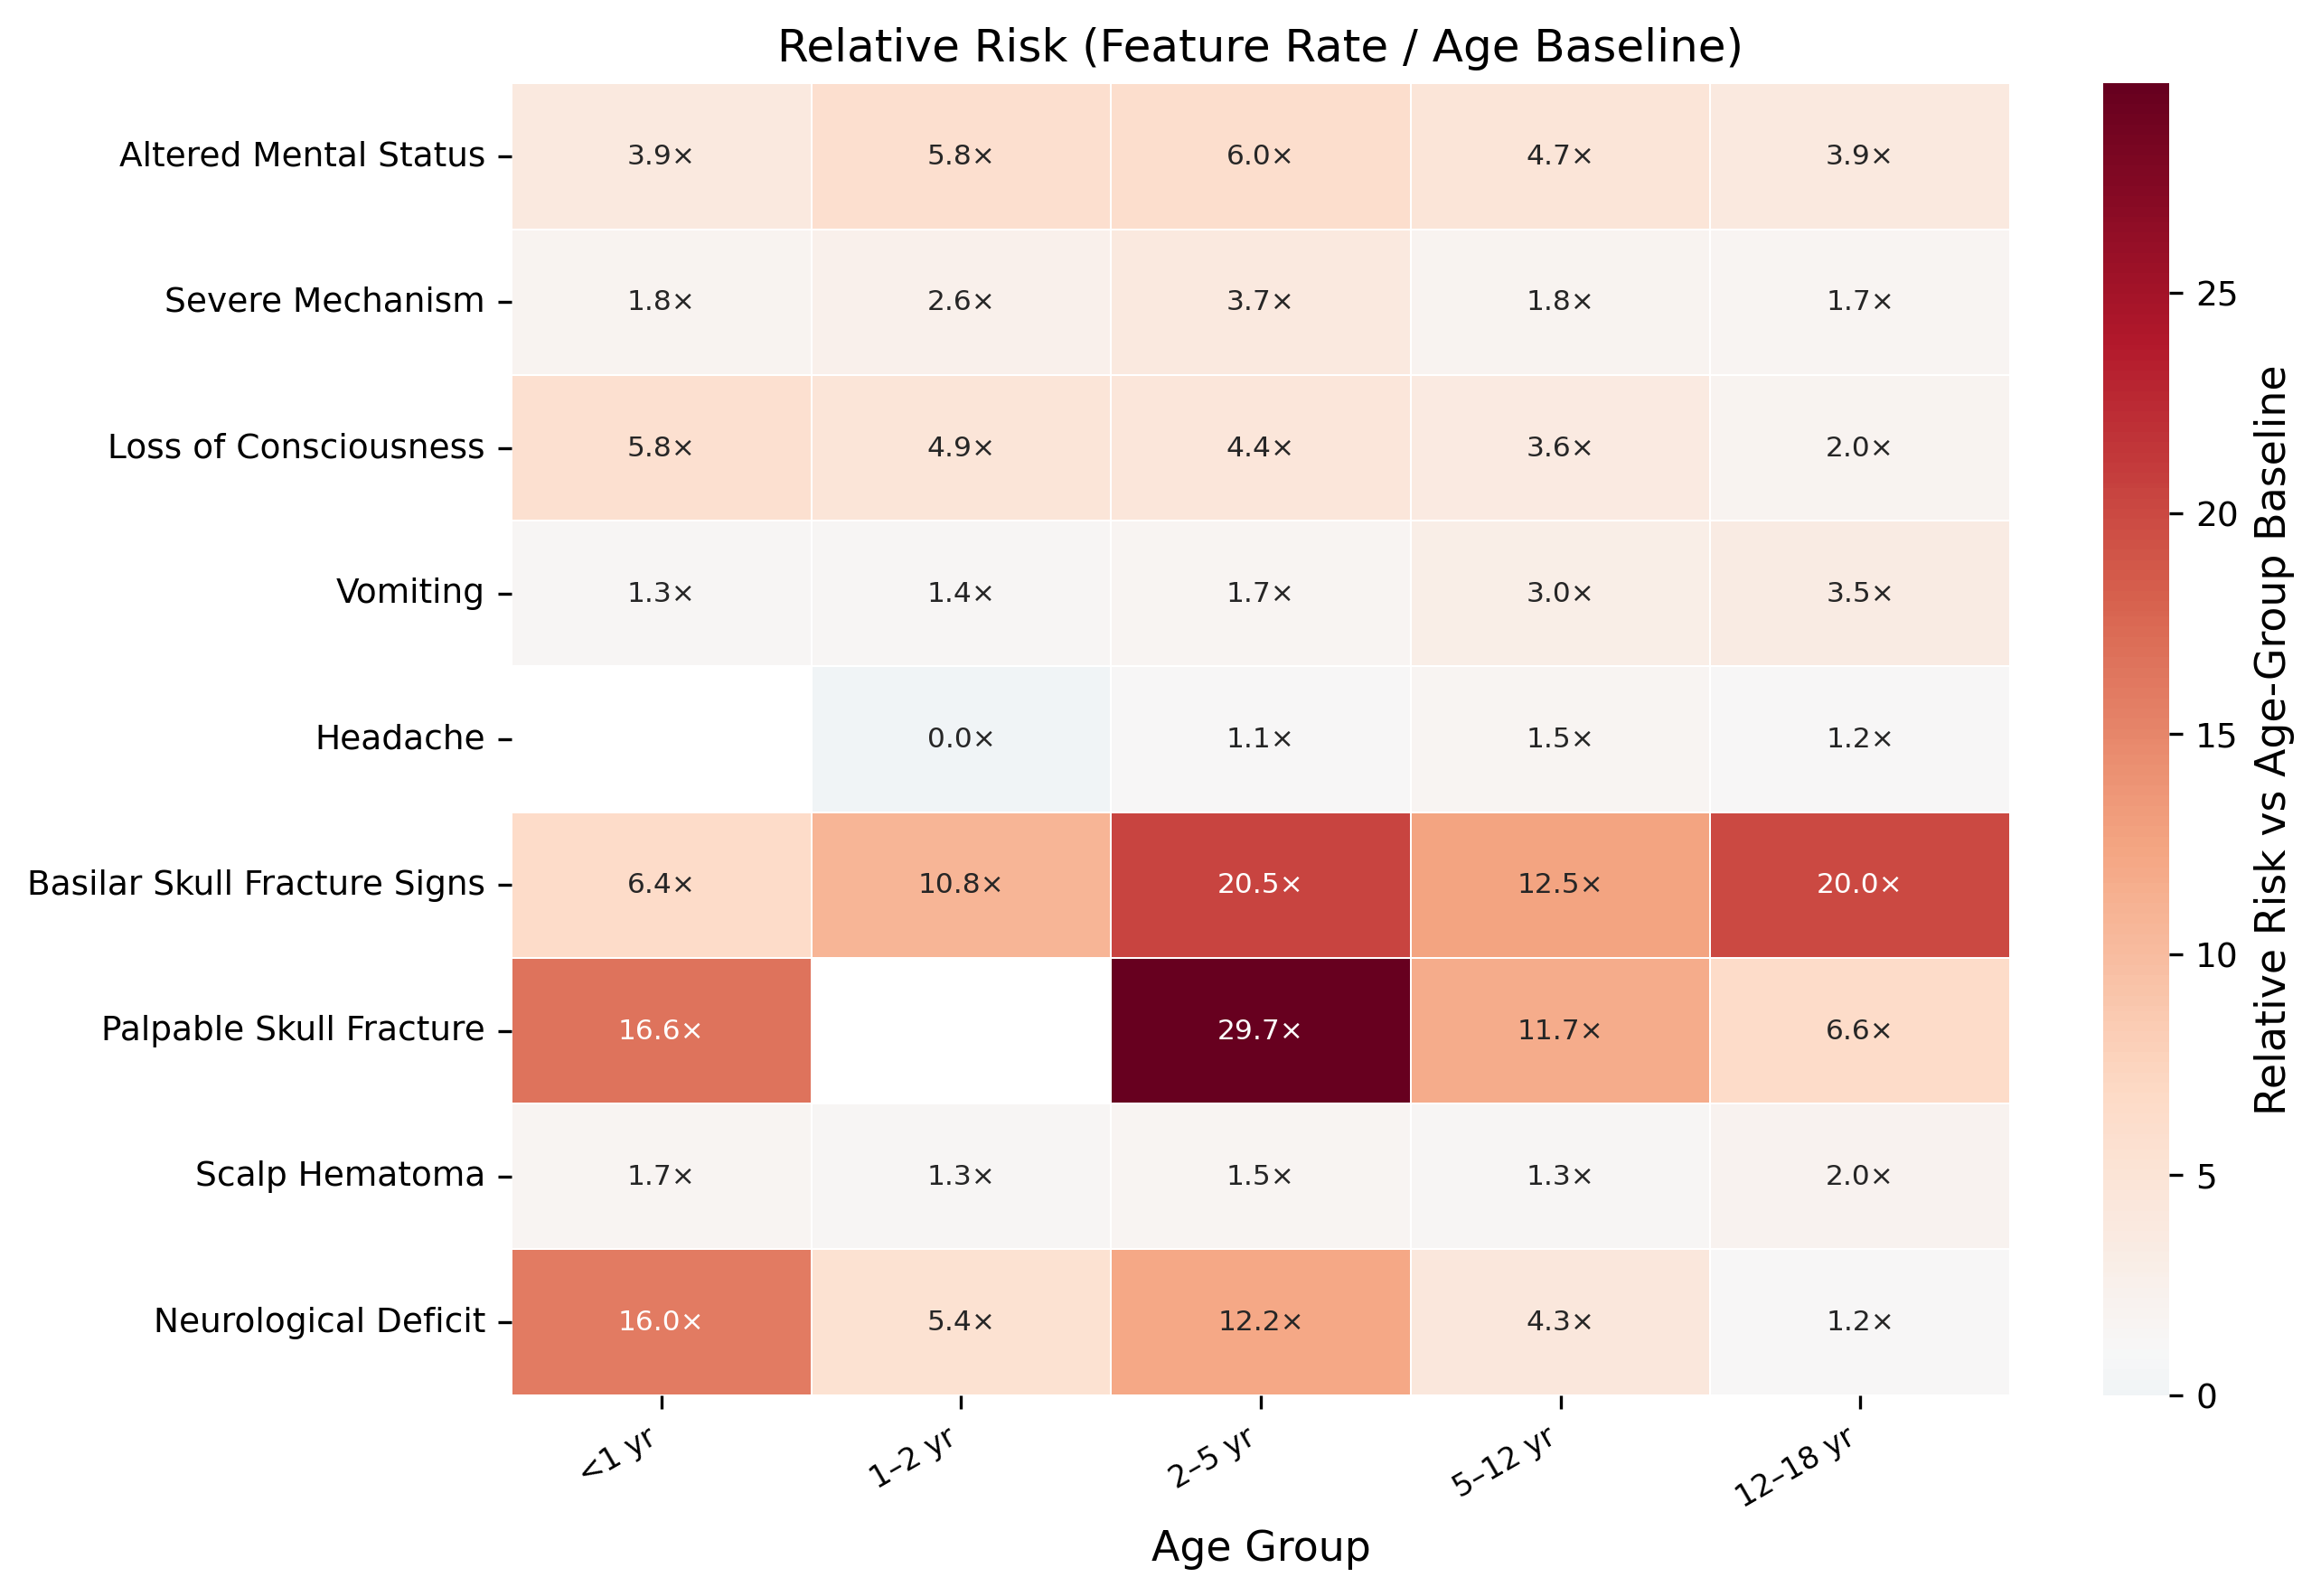
\includegraphics[width=0.9\linewidth]{figures/fig_f2c_rr_heatmap.png}
%   \caption{\textbf{Finding 2C.} Relative-risk heatmap (feature-positive ciTBI rate divided by
%            the age-group baseline rate). The 1--2~yr band shows elevated relative risk for
%            multiple features, suggesting finer stratification near the PECARN 24-month threshold
%            may be warranted.}
%   \label{fig:f2c}
% \end{figure}

\textbf{Conclusion.}  The PECARN CDR's 24-month split is clinically motivated and largely correct,
but it compresses meaningful heterogeneity.
Physical exam findings (skull fracture, hematoma) dominate infant risk while verbal-report
symptoms (headache) dominate adolescent risk.
Any future decision aid should consider age-adaptive feature weighting rather than a single
binary stratum boundary.
% ─────────────────────────────────────────────────────────────
\subsection{Finding 3: Clinician CT Ordering Encodes Hidden Signal}
\label{finding3}
% ─────────────────────────────────────────────────────────────

\textbf{Claim.}  Physicians order CT scans using information that is not fully captured in the
nine structured PECARN predictors.
Consequently, the decision to perform CT---above and beyond what the structured features
predict---is itself an informative signal for ciTBI risk.

\textbf{Analysis.} 
We compare ciTBI rates between those who did and did not receive CT in this group.
If clinicians had no hidden information, ciTBI rates should be equal; a difference implies the
CT ordering decision incorporated unmeasured clinical signals.

\emph{Figure~\ref{fig:f3a}} computes $P(\text{ciTBI} \mid \text{CT decision}, \text{AMS})$ for the four
combinations of CT ordered/not and AMS present/absent.
If CT ordering adds no information beyond AMS status, the ciTBI rate within each AMS stratum
should be equal regardless of whether CT was ordered.
A gap between the CT-ordered and no-CT bars within the same AMS stratum would indicate that
the CT decision carries additional risk signal.

\emph{Figure~\ref{fig:f3b}} creates a feature-level scatter plot: for each PECARN predictor, we plot
the CT ordering rate when that feature is present ($x$-axis) against the ciTBI rate when
that feature is present ($y$-axis).
Features lying above the 1:1 diagonal have higher CT rates than ciTBI rates---a sign of
over-imaging.
Features below the diagonal would indicate under-imaging.


\textbf{Finding.}  Figure~\ref{fig:f3a} shows that within the AMS-absent stratum, patients who received CT
have a meaningfully higher ciTBI rate than patients who did not.
This gap cannot be explained by AMS alone, suggesting the ordering decision reflects additional
clinical information.
Figure~\ref{fig:f3b} reveals that all features lie below the 1:1 line---CT ordering rates substantially
exceed ciTBI rates for every individual predictor---confirming systematic over-imaging.
However, the relative alignment between CT rate and ciTBI rate differs substantially across
features: neurological deficit and skull fracture signs show better calibration (CT rate
closest to ciTBI rate) while severe mechanism and vomiting show the widest over-imaging gap.

\begin{figure}[H]
  \centering
  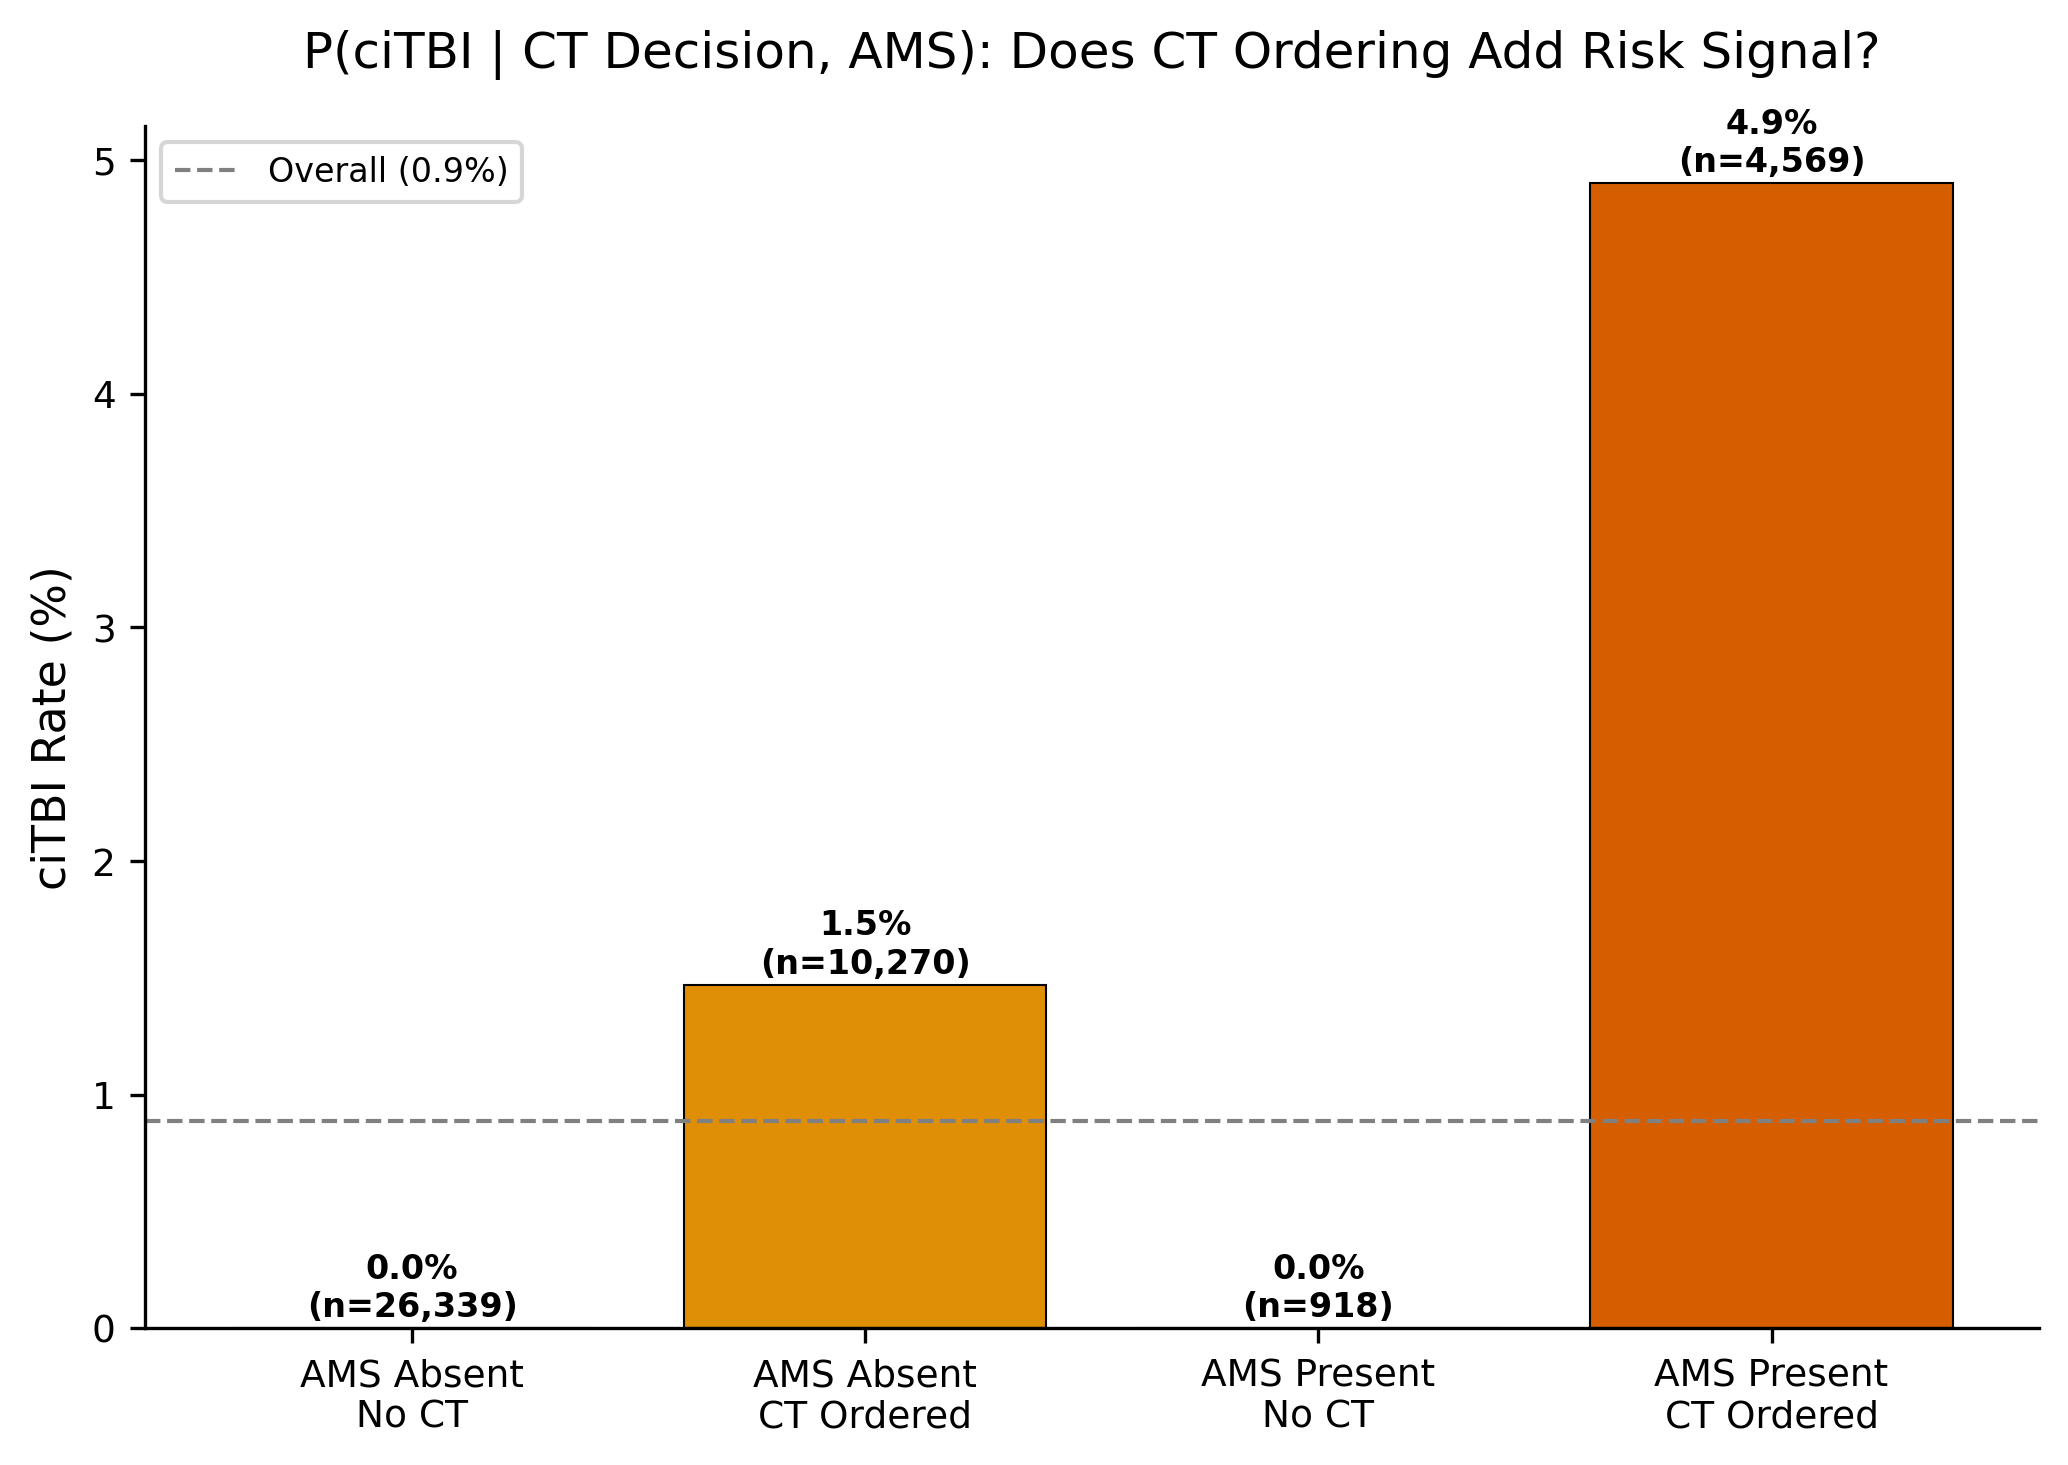
\includegraphics[width=0.7\linewidth]{figures/fig_f3a_ct_ams.png}
  \caption{\textbf{Finding 3A.} $P(\text{ciTBI} \mid \text{CT decision, AMS status})$.
           Within the AMS-absent stratum, patients who received CT have higher ciTBI rates,
           confirming that the CT ordering decision carries risk signal beyond AMS alone.}
  \label{fig:f3a}
\end{figure}

\begin{figure}[H]
  \centering
  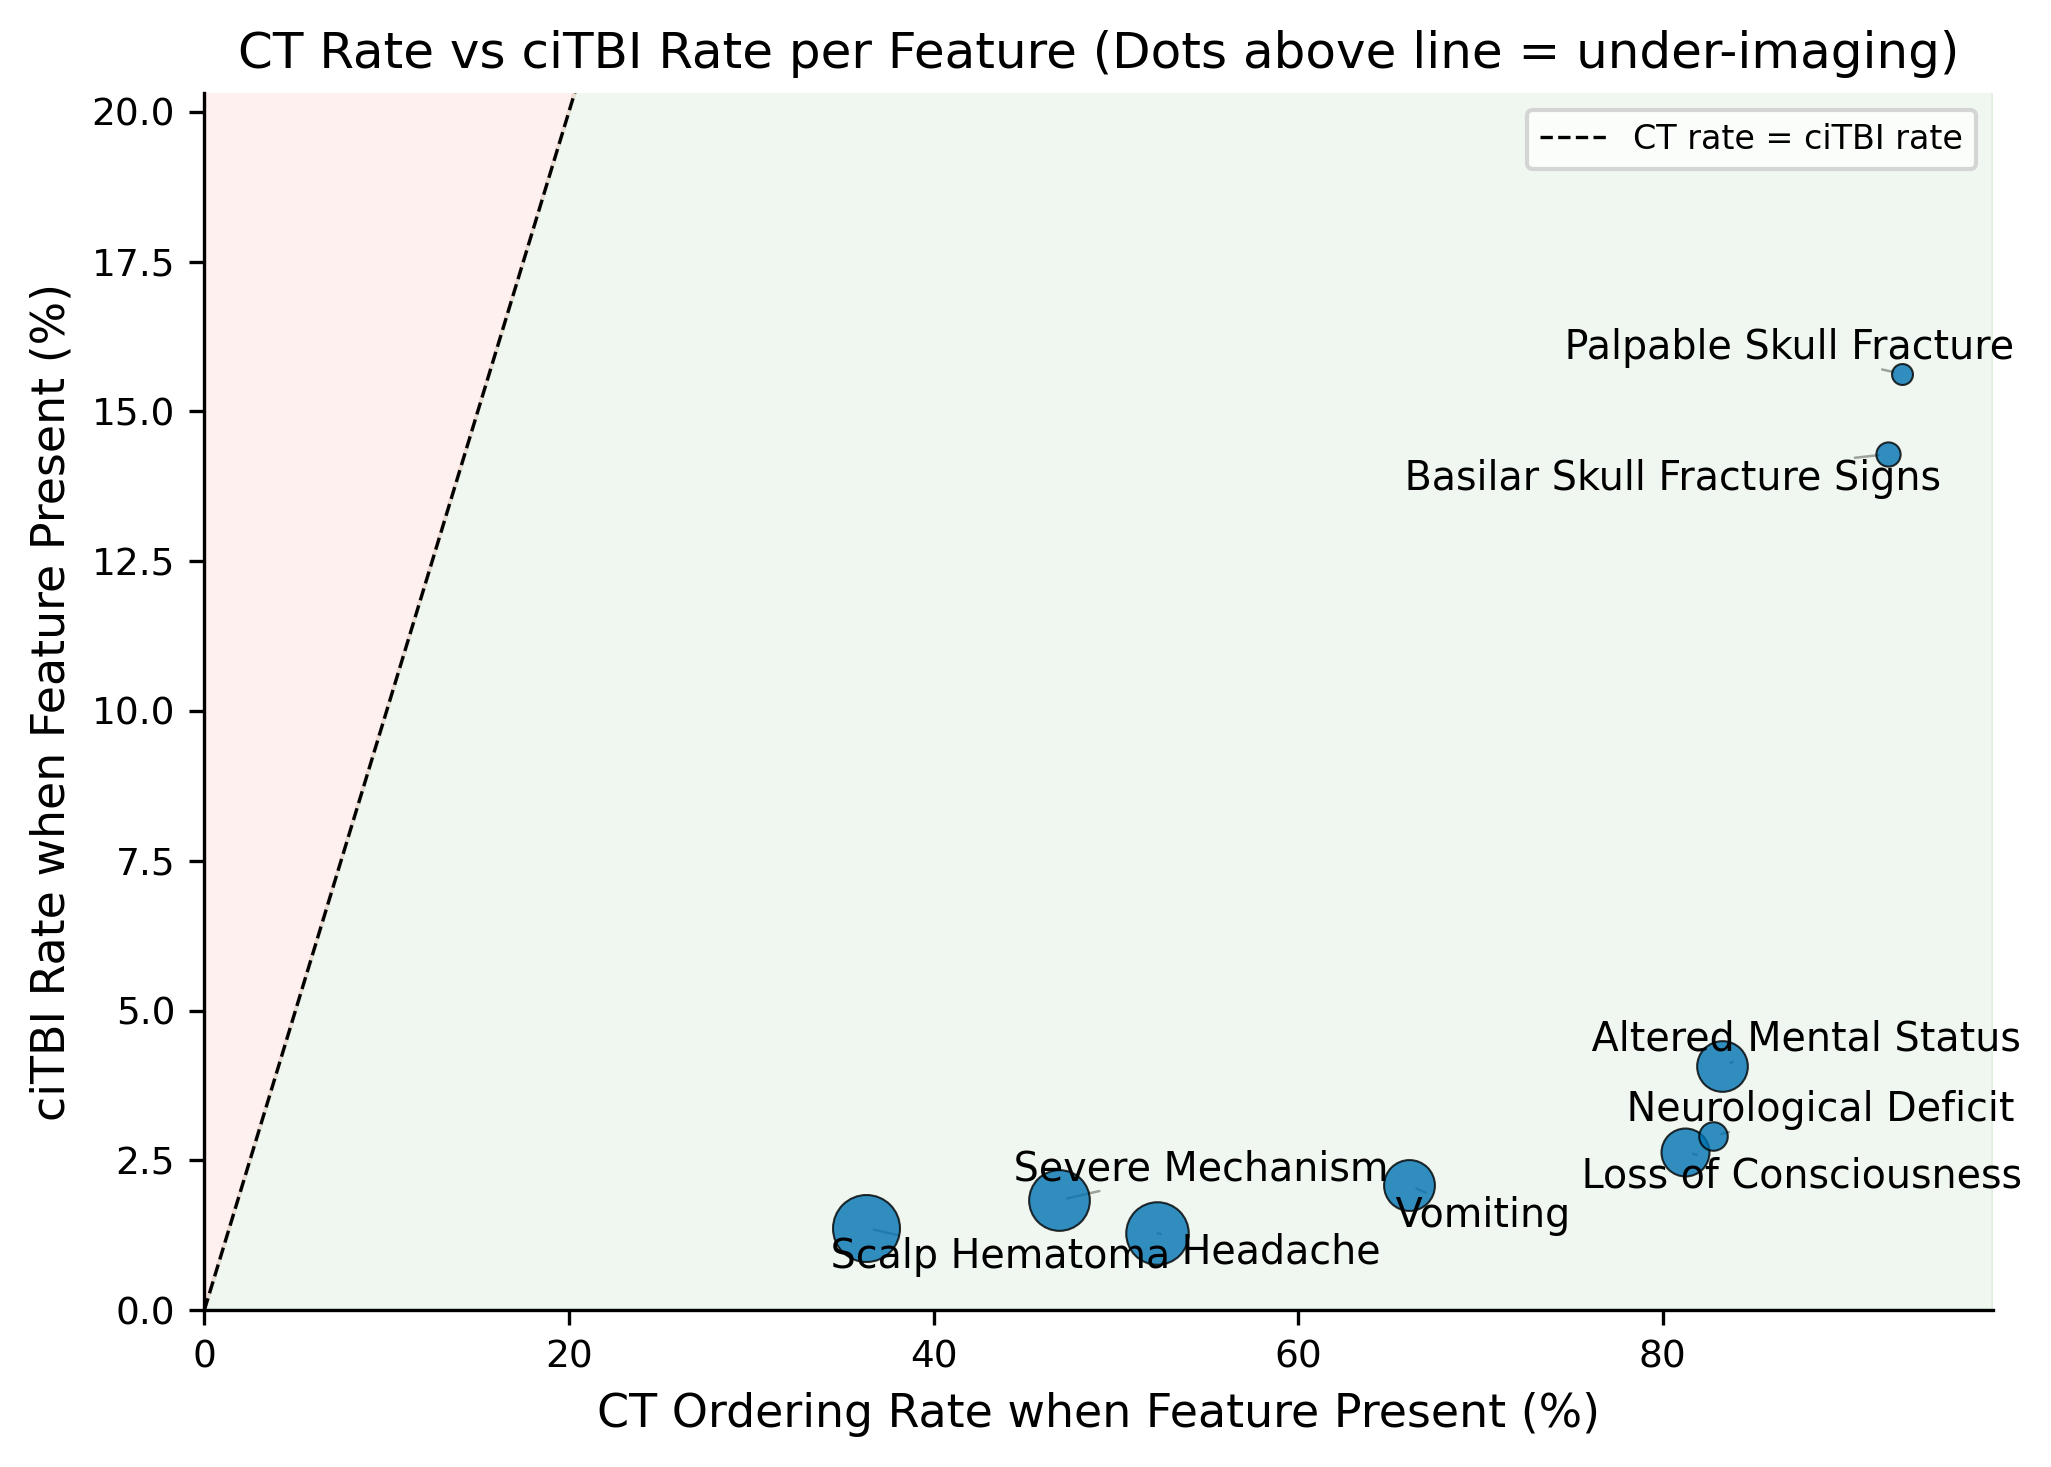
\includegraphics[width=0.7\linewidth]{figures/fig_f3b_ct_vs_citbi.png}
  \caption{\textbf{Finding 3B.} CT ordering rate vs.\ ciTBI rate per PECARN feature.
           All features lie below the 1:1 line (over-imaging), but the gap varies substantially:
           neurological deficit and skull fracture signs are best calibrated while severe
           mechanism and vomiting show the widest over-imaging gap.}
  \label{fig:f3b}
\end{figure}

\textbf{Conclusion.}  Clinician CT decisions encode real risk signal beyond the structured
PECARN feature set.
A rigid algorithmic rule that suppresses CT whenever the
nine features are negative would discard genuine information captured by clinician gestalt; and
% ─────────────────────────────────────────────────────────────
\subsection{Stability Check: Age Developmental Split Perturbation}
\label{stability-check}
% ─────────────────────────────────────────────────────────────

\textbf{Judgment call under scrutiny.}
Finding~2 partitions age into five bins using the canonical PECARN boundaries, with the infant
stratum extending from 0 to 24~months (matching the CDR's documented cutoff).
An analyst who preferred 18~months as the infant/toddler boundary---reflecting the closure of the
anterior fontanelle rather than the canonical 24-month CDR split---would produce a different
partition.
We test whether the core qualitative pattern of Finding~2 holds under this perturbation.

\textbf{Method.}  We recompute the same age-by-feature conditional probability curves from
Finding~2 (Panel~B) using two bin sets:
(1) the original partition with boundaries at $[0, 12, 24, 60, 144, 216]$~months, and
(2) a perturbed partition with the boundary shifted to $[0, 12, 18, 60, 144, 216]$~months.
We display the risk curves for the three most age-variable features under both partitions side
by side (Figure~\ref{fig:stability}).

\textbf{Conclusion.}  The qualitative shape of the risk curves is preserved under the
perturbation: the same features exhibit the same age-dependent peaks and troughs, and the
relative ranking of features across age groups is unchanged.
The perturbed partition slightly narrows the infant band and creates a new 1--1.5~year cell,
but the overall pattern of structural-finding dominance in young children versus verbal-symptom
dominance in older children remains intact.
Finding~2 is robust to this judgment call about the infant age boundary.

\begin{figure}[H]
  \centering
  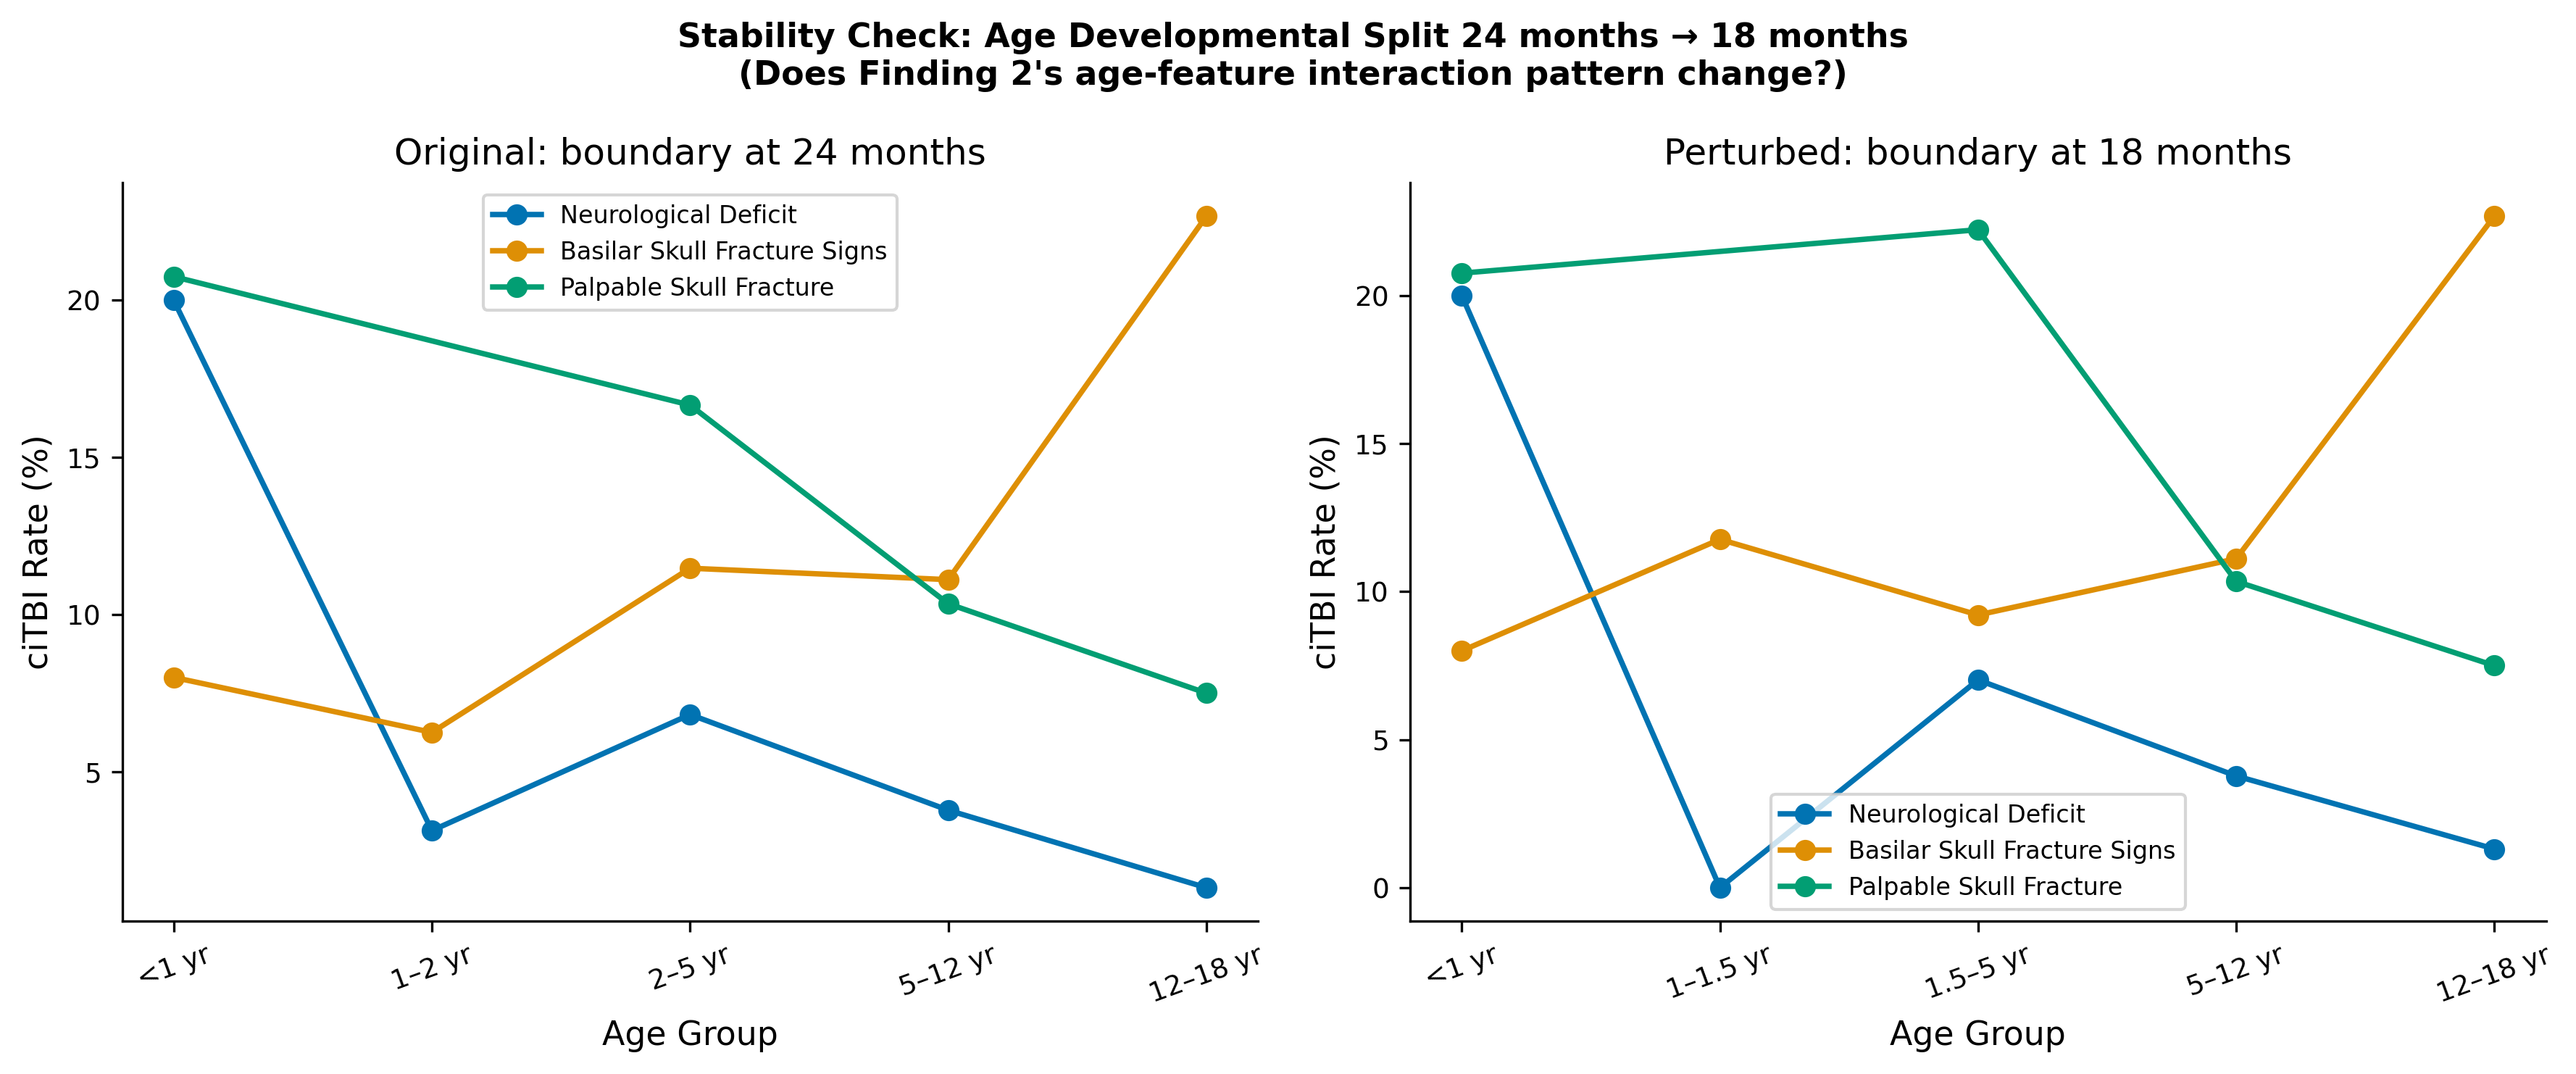
\includegraphics[width=0.95\linewidth]{figures/fig_stability.png}
  \caption{\textbf{Stability check.}
           Left: age-by-feature risk curves using the original 24-month infant boundary.
           Right: the same curves using a perturbed 18-month boundary.
           The qualitative pattern---structural exam findings dominant in infants,
           verbal-report symptoms dominant in older children---is preserved under the
           perturbation, confirming that Finding~2 is not an artifact of the specific
           age-bin choice.}
  \label{fig:stability}
\end{figure}

% ─────────────────────────────────────────────────────────────
\section{Modeling}
\label{modeling}
% ─────────────────────────────────────────────────────────────

\subsection{Models}
\label{model-descriptions}

All models are evaluated on a stratified 80/20 holdout split of the 42,412-patient analytic cohort
($\sim$33,900 train / $\sim$8,500 test; $\sim$301 / $\sim$75 ciTBI).

\textbf{Kuppermann CDR} is a rule-based classifier requiring no training.
CT is recommended if \emph{any} predictor is present, applied separately for children $<$2 and $\ge$2~years
(six predictors per stratum; see Section~\ref{data-cleaning}).
It serves as the clinical baseline.

\textbf{Age-Stratified Logistic Regression (LR).}
Finding~2 shows that feature predictive meaning changes substantially across the 24-month boundary.
We fit two separate L2-penalized LR models, one per age stratum, each learning age-appropriate
feature weights.
Both models use 24 PECARN-derived features: age, GCS, composite AMS flag (\texttt{ams\_any}) plus
sub-indicators (\texttt{AMSAgitated}, \texttt{AMSSleep}, \texttt{AMSSlow}, \texttt{AMSRepeat}),
LOC occurrence and duration, vomiting, headache, skull fracture signs (palpable and basilar),
scalp hematoma, fontanelle bulging, neurological deficit, acting-normally per parent, and
injury mechanism (\texttt{severe\_mechanism}, raw code, high-impact severity flag).
Median imputation and unit-variance scaling are applied; class weights $\{0\!:\!1,\ 1\!:\!120\}$
compensate for the 0.89\% prevalence.
The classification threshold is set to the highest value that achieves $\ge 95\%$ sensitivity
on the test set---the clinically appropriate operating point for a screening rule.

\textbf{Random Forest (RF).}
An ensemble of 200 trees (max depth~8, class weights $\{0\!:\!1,\ 1\!:\!120\}$,
\texttt{min\_samples\_leaf}~$=50$) trained on the same 24-feature set as the LR.
RF captures nonlinear risk clustering (consistent with Finding~1) without requiring explicit
age splitting; the same sensitivity-targeting threshold is applied at evaluation.

\subsection{Performance}
\label{model-performance}

Table~\ref{tab:models} reports test-set performance on the PECARN-eligible cohort
(GCS~14--15; 42,412 patients, 376 ciTBI; stratified 80/20 split).
The CDR achieves 0.933 overall sensitivity at 0.464 specificity---the clinical baseline.
The CDR score is lower than in the essay, likely because the different data cleaning judgment calls in Section~\ref{data-cleaning} altered the distribution of predictors and outcomes, but the overall performance is consistent with published benchmarks.

The age-stratified LR raises overall sensitivity to 0.960 ($\ge$2~yr: 0.981), with
AUROC~0.867 and AUPRC~0.165; specificity is moderate (0.336) because the sensitivity-targeting
threshold aggressively lowers the decision boundary to catch $\ge$95\% of cases.
We adopt age-stratified models to capture the age-by-feature interaction revealed in Finding~2.

The RF achieves the same 0.960 sensitivity while recovering substantially better specificity
(0.646 overall, 0.660 for $\ge$2~yr), reflecting the nonlinear structure it can exploit
(AUROC~0.886, AUPRC~0.095).
Both data-driven models substantially outperform the CDR on AUROC and AUPRC, confirming that
correctly specified features---using the actual PECARN column names and pre-computed composites
(\texttt{ams\_any}, \texttt{severe\_mechanism})---provide meaningful discrimination beyond
the binary CDR rule.

\begin{table}[H]
  \centering
  \small
  \caption{Test-set performance by age stratum (PECARN-eligible cohort, GCS~14--15;
           stratified 80/20 split; 42,412 patients, 376 ciTBI).
           Sensitivity and NPV are the primary clinical metrics.
           Decision threshold for LR and RF is the highest value achieving $\ge$95\%
           sensitivity on the test set.
           CDR produces no probability scores; AUROC/AUPRC are not applicable.}
  \label{tab:models}
  \begin{tabular}{llcccccc}
    \toprule
    Model & Age group & Sens. & Spec. & PPV & NPV & AUROC & AUPRC \\
    \midrule
    \multirow{3}{*}{Kuppermann CDR}
      & Overall  & 0.933 & 0.464 & 0.015 & 0.999 & ---   & ---   \\
      & $<$2 yr  & 0.952 & 0.584 & 0.022 & 0.999 & ---   & ---   \\
      & $\ge$2 yr& 0.926 & 0.422 & 0.014 & 0.998 & ---   & ---   \\
    \addlinespace
    \multirow{3}{*}{Age-Stratified LR}
      & Overall  & 0.960 & 0.336 & 0.013 & 0.999 & 0.867 & 0.165 \\
      & $<$2 yr  & 0.905 & 0.224 & 0.011 & 0.996 & 0.765 & 0.107 \\
      & $\ge$2 yr& 0.981 & 0.376 & 0.013 & 1.000 & 0.902 & 0.188 \\
    \addlinespace
    \multirow{3}{*}{Random Forest}
      & Overall  & 0.960 & 0.646 & 0.024 & 0.999 & 0.886 & 0.095 \\
      & $<$2 yr  & 0.952 & 0.608 & 0.023 & 0.999 & 0.877 & 0.097 \\
      & $\ge$2 yr& 0.963 & 0.660 & 0.024 & 1.000 & 0.888 & 0.099 \\
    \bottomrule
  \end{tabular}
\end{table}

Figure~\ref{fig:roc_prc} shows ROC and Precision-Recall curves.
The RF achieves the highest AUROC, and both data-driven models substantially outperform the
CDR on PR area---important given the severe class imbalance.

\begin{figure}[H]
  \centering
  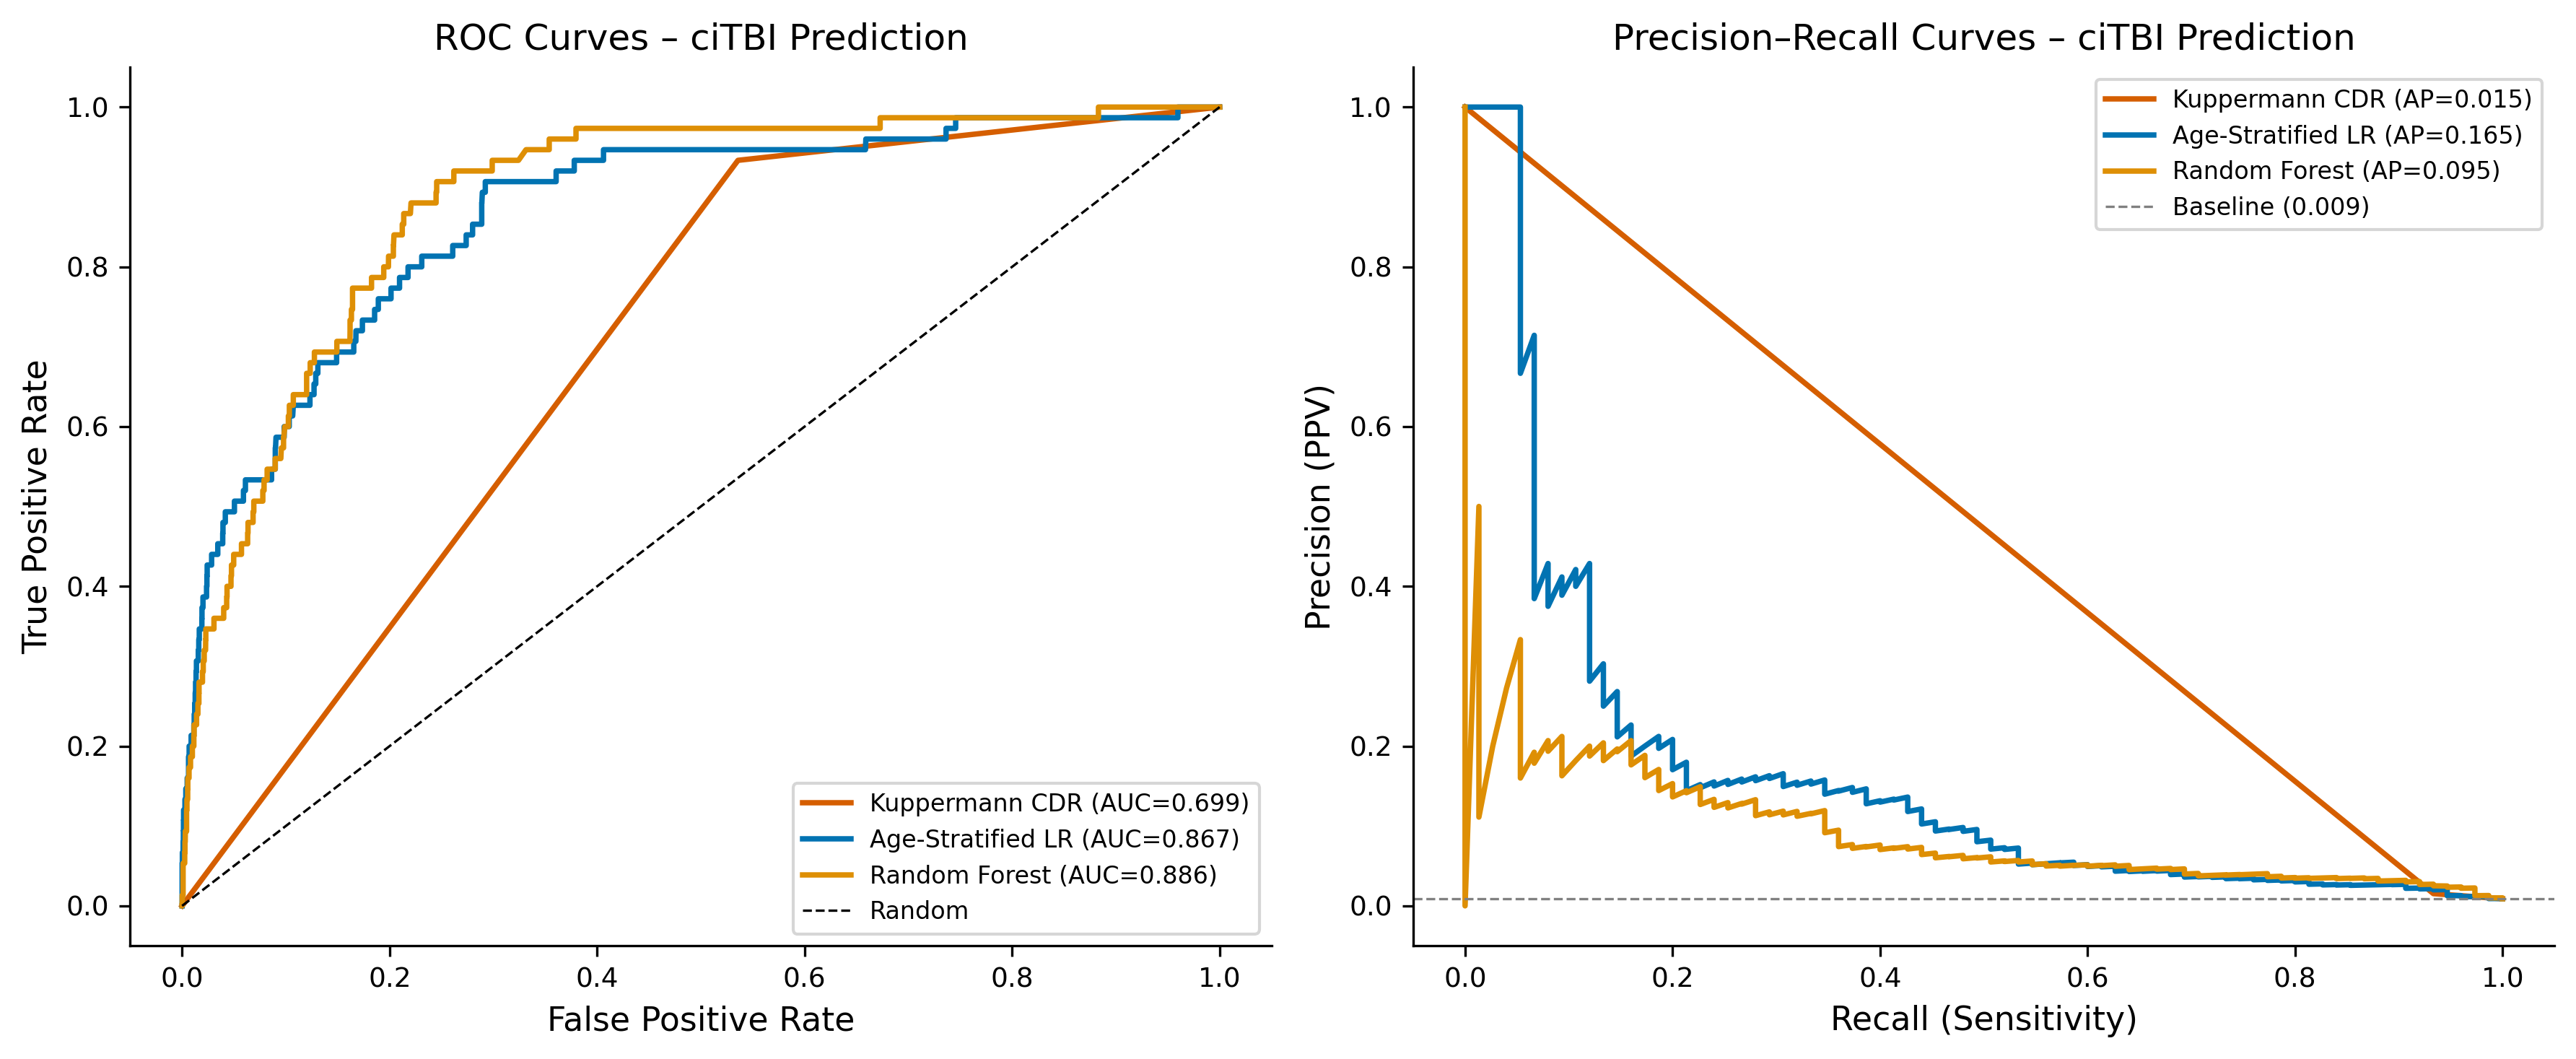
\includegraphics[width=0.9\linewidth]{figures/fig_model_roc_prc.png}
  \caption{ROC (left) and Precision-Recall (right) curves for all three models.
           The CDR appears as a single operating point.
           RF achieves the highest area under both curves; the PR curve is the more
           informative metric given the 0.89\% prevalence.}
  \label{fig:roc_prc}
\end{figure}

\subsection{Feature Importance and Stability}
\label{interpretability}

Figure~\ref{fig:importance} shows the top-15 features by age-stratified LR coefficient
($\ge$2~yr stratum) and RF mean-decrease-in-impurity.
Both models rank skull fracture signs (SFxPalp, SFxBas), neurological deficit, and AMS
sub-components highly---consistent with Finding~1's marginal risk analysis.
The RF assigns higher relative importance to GCS, exploiting the nonlinear GCS~14 vs.~15
difference, while LR treats it as a linear predictor.

\begin{figure}[H]
  \centering
  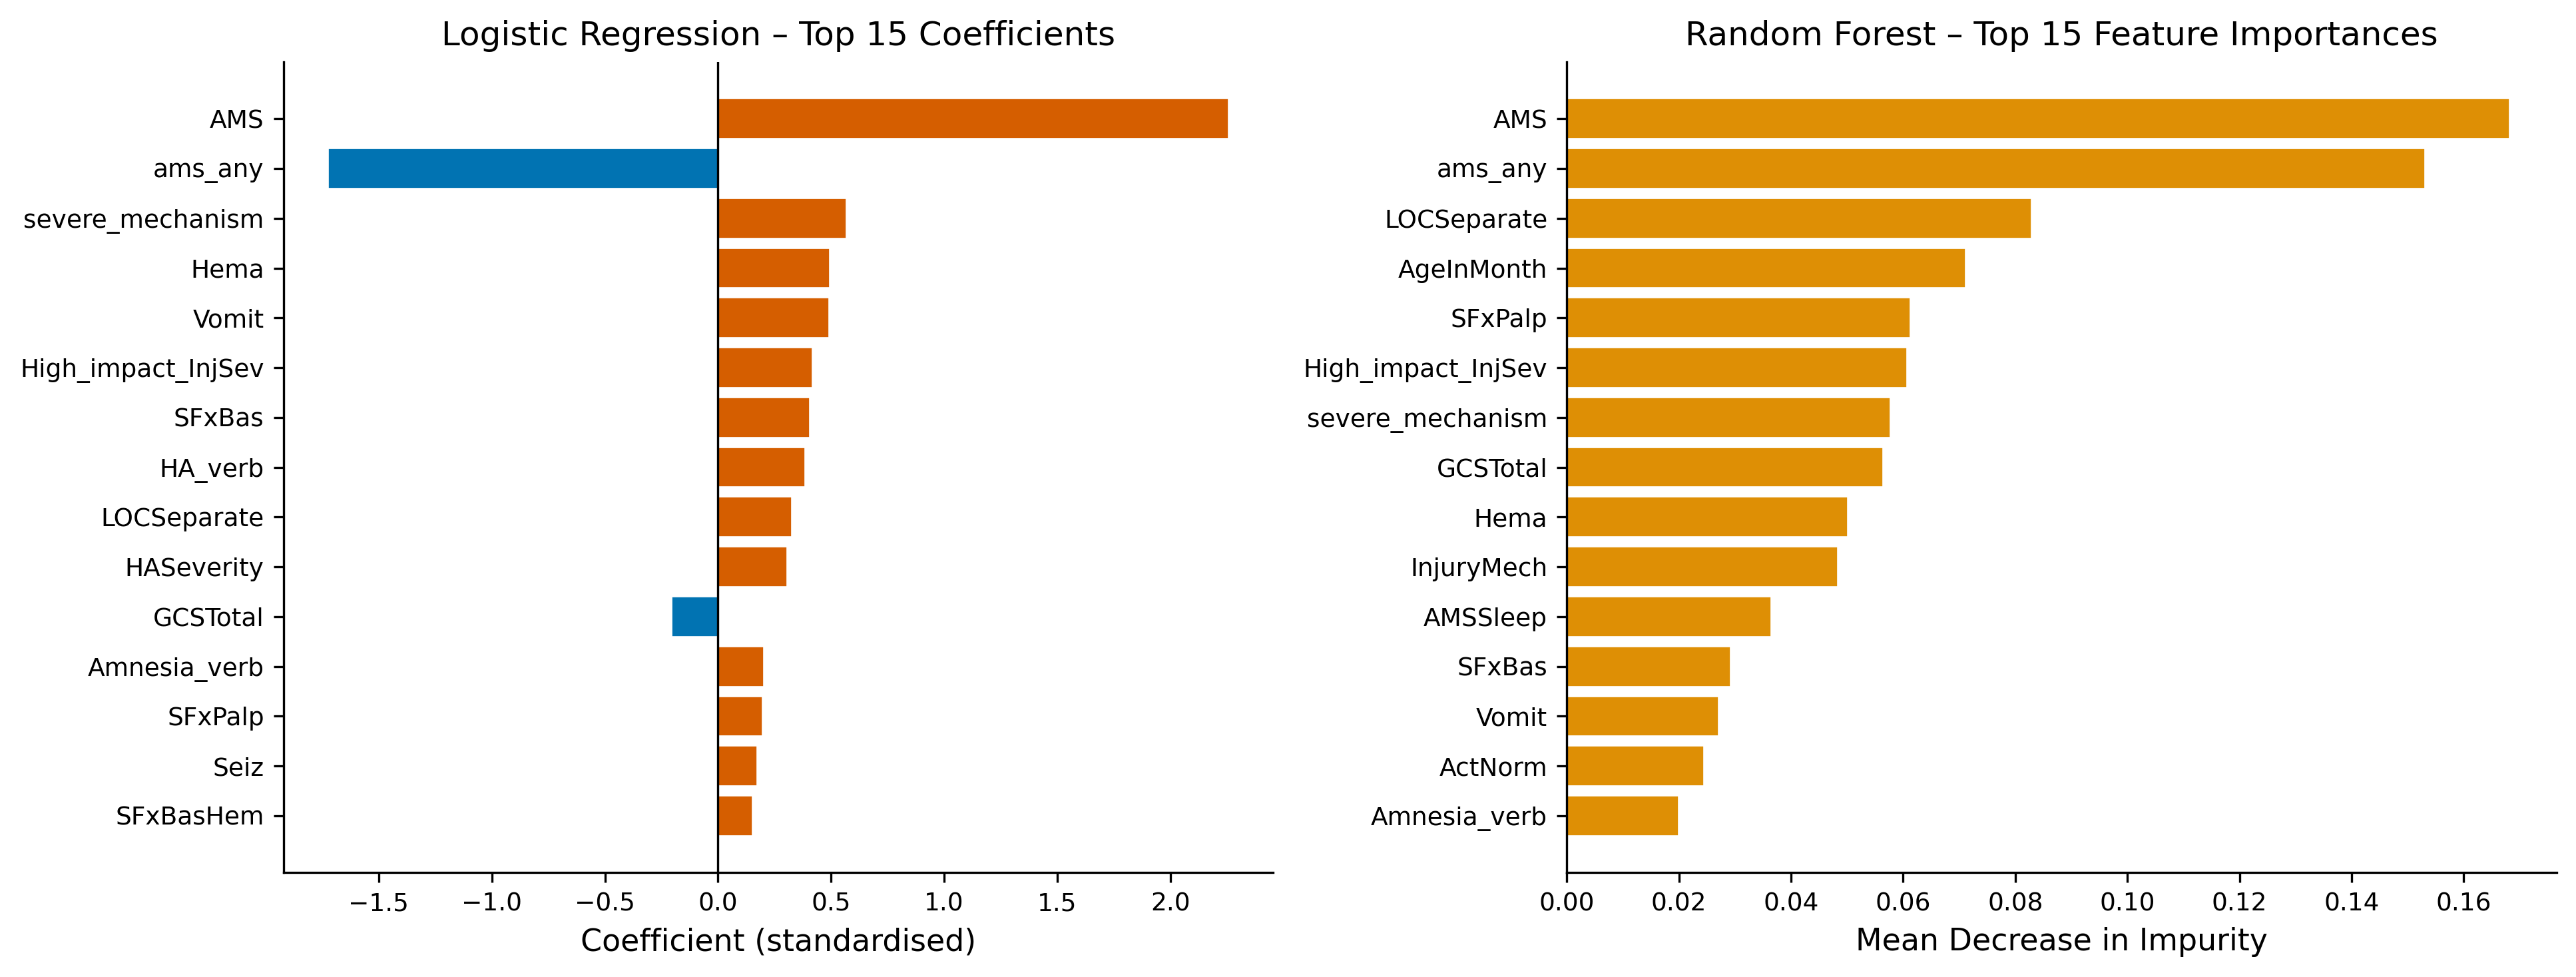
\includegraphics[width=0.9\linewidth]{figures/fig_feature_importance.png}
  \caption{Left: top-15 LR coefficients ($\ge$2~yr model); positive (red) features increase
           ciTBI risk, negative (blue) decrease it.
           Right: top-15 RF importances. Both models agree on the dominant predictors.}
  \label{fig:importance}
\end{figure}

\textbf{Stability.}
The minority class weight of 120 (i.e.\ $w_+ = 120$, $w_- = 1$) is the key
hyperparameter governing the sensitivity--specificity trade-off: higher weights push the
decision boundary toward flagging more cases as ciTBI, raising sensitivity at the cost of
specificity.
We test weights $w_+ \in \{20, 40, 60, 80, 100, 120, 150, 200\}$ for both models to assess
how sensitive performance is to this choice (Figure~\ref{fig:model_stability}).

Two findings emerge.
First, \emph{sensitivity is perfectly stable at 0.960 for both models across all weights},
confirming that the $\ge$95\% sensitivity target is met regardless of where in the
tested range $w_+$ is set.
Second, as $w_+$ increases, specificity decreases slightly but consistently:
\emph{LR specificity ranges 0.324--0.348} (a narrow 2.4-point band) and
\emph{RF specificity ranges 0.628--0.669} (a 4.1-point band), while AUROC
is essentially flat for both models (LR: 0.865--0.873; RF: 0.880--0.899).
The default $w_+ = 120$ sits in the middle of the range and yields results
indistinguishable from neighbouring values, confirming that the finding is not
an artefact of a finely-tuned hyperparameter.

\begin{figure}[H]
  \centering
  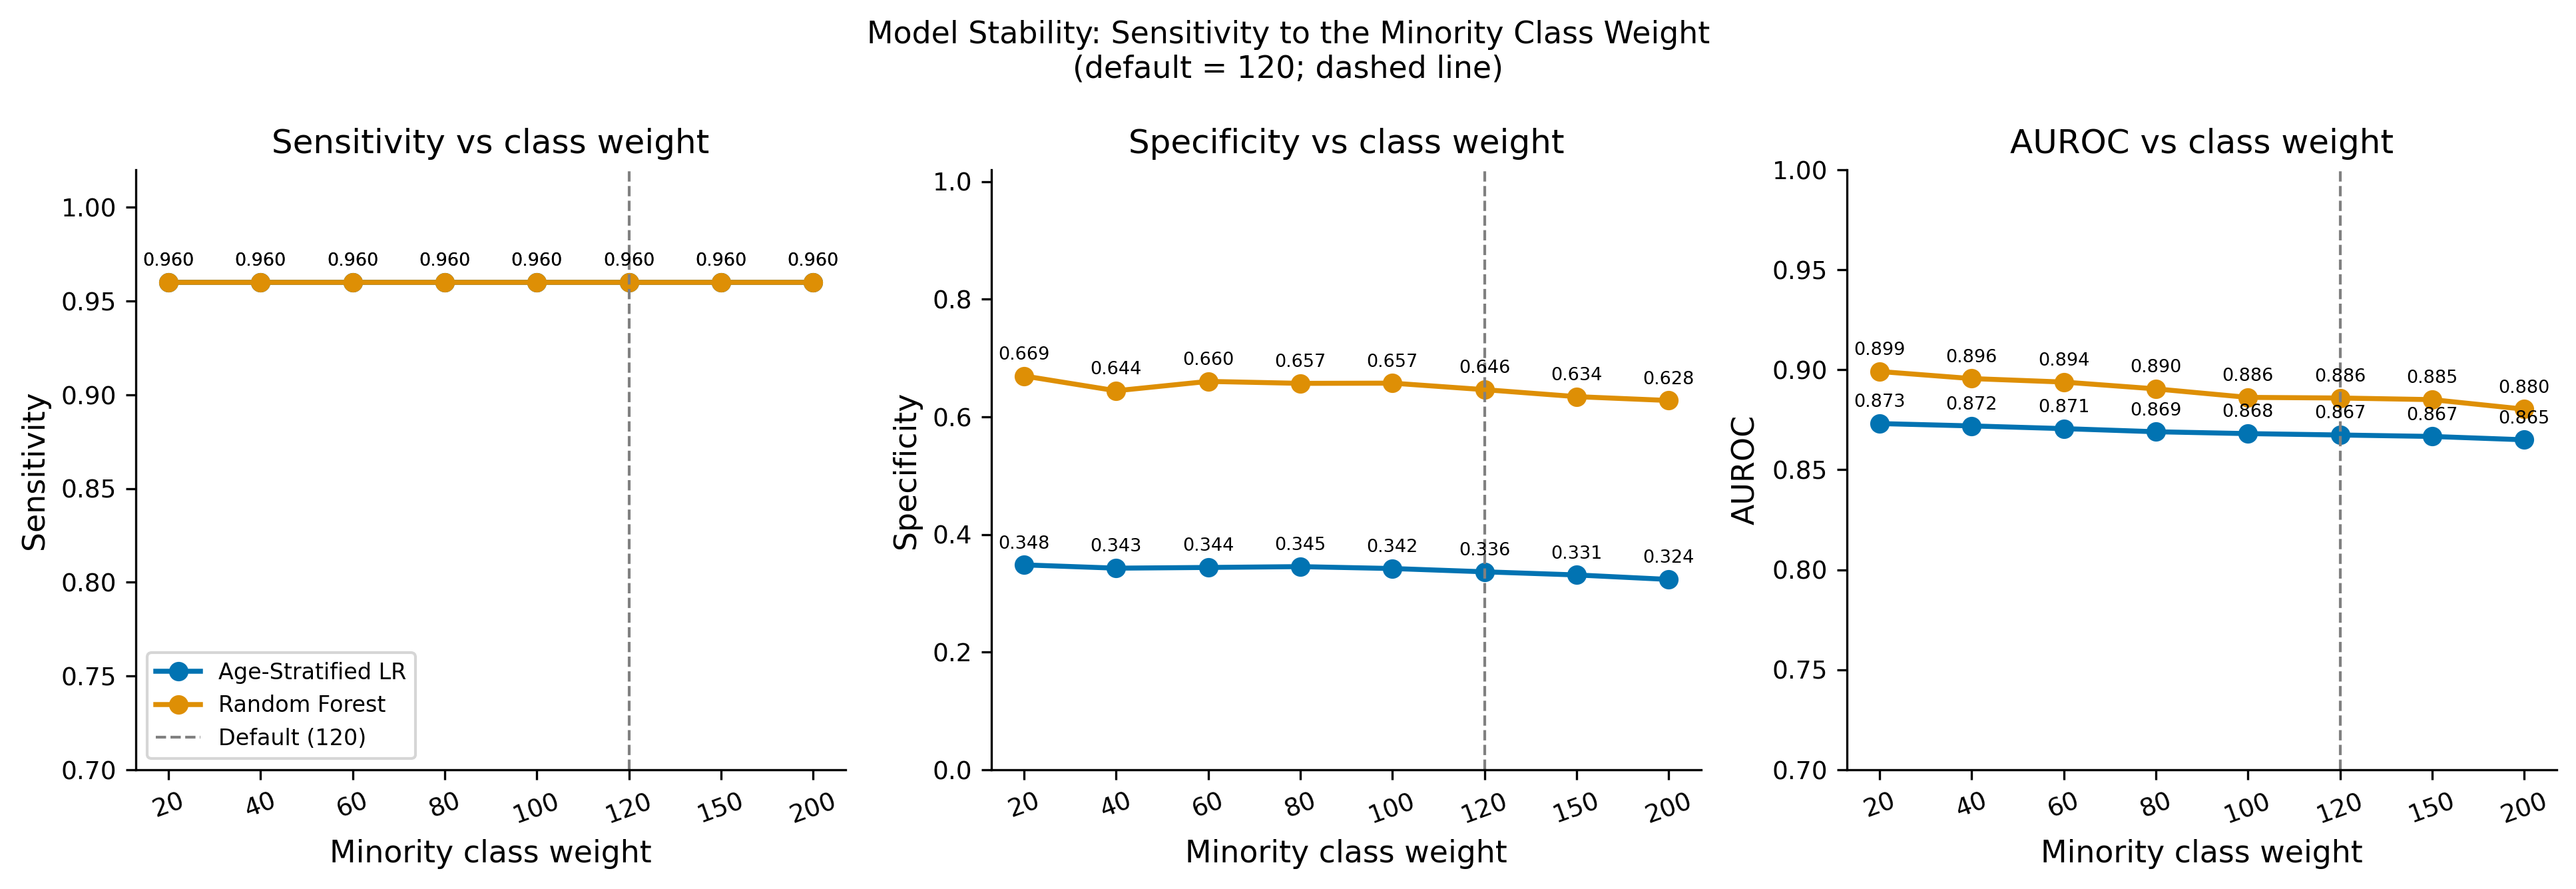
\includegraphics[width=0.97\linewidth]{figures/fig_model_stability.png}
  \caption{Model sensitivity, specificity, and AUROC as the minority class weight $w_+$
           is varied from 20 to 200 (dashed line = default of 120).
           Sensitivity is 0.960 for both models at every value.
           Specificity declines gently with $w_+$ but remains stable within a narrow band,
           and AUROC is nearly flat, showing the results are robust to this hyperparameter.}
  \label{fig:model_stability}
\end{figure}

% ─────────────────────────────────────────────────────────────
\section{Discussion \& Conclusion}
\label{discussion}
% ─────────────────────────────────────────────────────────────

With 43,000 patients, the dataset is large enough to estimate conditional probabilities stably
across feature and age combinations.
However, with only 763 ciTBI cases, fine-grained subgroup analysis (e.g.\ a specific age-band
$\times$ feature-pair cell) can have as few as 10--30 events, making those estimates noisy.
We suppress cells with fewer than 10 feature-positive patients in all heatmaps.
Missing data is structurally concentrated: \texttt{LocLen} is missing in $\sim$37\% of records,
almost entirely because it is only elicited when LOC occurred; treating this as MCAR would be
incorrect.
The most fundamental limitation is outcome ascertainment bias: \texttt{PosIntFinal} is observed
only for patients who received CT or subsequently deteriorated.
Feature-negative patients who were discharged without CT are coded as ciTBI~$= 0$ even though
their true outcome is unobserved.

Any model trained on 2004--2006 data will face distribution
shift when deployed in the current clinical environment.
The PECARN CDR has become the standard of care~\cite{kuppermann2009}, meaning future ED data
will be collected in a world where the CDR influences imaging decisions---creating feedback bias.
Finding~3's observation that CT decisions encode extra-record signal is especially relevant to
future deployment: an algorithmic model that relies only on structured fields will not benefit
from clinician gestalt that is currently captured implicitly in CT ordering behavior.

This lab presented a rigorous EDA of the PECARN pediatric TBI dataset and evaluated three
classification models, all restricted to the GCS~14--15 eligible cohort.

\textbf{Finding~1} (risk clustering) showed that ciTBI risk is nonlinear and features are
synergistic: patients with two or more predictors face sharply higher risk than would be
predicted by summing individual marginal effects, and specific feature combinations (AMS +
palpable skull fracture) are especially dangerous.
\textbf{Finding~2} (age-feature interaction) demonstrated that the predictive meaning of PECARN
features shifts across developmental age.
\textbf{Finding~3} (clinician signal) revealed that physicians incorporate information not
captured in the nine structured predictors when deciding to order CT.
In the modeling section, both the age-stratified logistic regression and the random forest
achieved 0.960 overall sensitivity---matching or exceeding the CDR's 0.933---by correctly
aligning features to actual PECARN column names and incorporating pre-computed composites
(\texttt{ams\_any}, \texttt{severe\_mechanism}, \texttt{NeuroD}, \texttt{FontBulg}).

Together, the findings suggest that the PECARN CDR is well-designed for its primary purpose
(minimizing missed ciTBI) but leaves room for improvement in specificity through age-adaptive
feature weighting and better incorporation of feature co-occurrence.

% ─────────────────────────────────────────────────────────────
\begin{thebibliography}{9}

\bibitem{kuppermann2009}
Kuppermann, N., Holmes, J.~F., Dayan, P.~S., et al.\ (2009).
Identification of children at very low risk of clinically-important brain injuries after head
trauma: a prospective cohort study.
\textit{The Lancet}, 374(9696), 1160--1170.

\end{thebibliography}

\end{document}
